\documentclass[10pt,letterpaper]{phstylee} %,twoside]{phstylee}

\usepackage[latin1]{inputenc}
\usepackage[spanish]{babel}
\usepackage{amsmath}
%\usepackage[T1]{fontenc}
\usepackage[dvips,final]{epsfig}
\usepackage{setspace}
\usepackage{amssymb}
\usepackage{cite}
\usepackage{amsfonts}
\usepackage{amsxtra}

\usepackage{times}
\usepackage{float}
\usepackage{eso-pic}
\usepackage{multicol}
\usepackage{enumerate}
\usepackage{url}
\usepackage{soul}
%\usepackage{fancyhdr}

\usepackage{color}
\usepackage{graphicx}

\usepackage{enumitem}
%\usepackage[table]{xcolor}
\usepackage{multirow}
\usepackage{caption}
\usepackage{subcaption}
\usepackage{gensymb}
\usepackage{listings}

\allowdisplaybreaks

%%%%%%%%%%%%%%%%%%%%%
%      DIRECTORIO DONDE BUSCA LAS FIGURAS

%\graphicspath{{fig/}}

% Pre\'ambulo
\newcommand{\ltr}[1]{\ensuremath{{\cal{L}}\left[#1\right]}} %Laplace transform
\newcommand{\ztr}[1]{\ensuremath{{\cal{Z}}\left\lbrace #1 \right\rbrace }} %zeta transform
\newcommand{\matriz}[1]{\left[\begin{matrix}#1\end{matrix}\right]}
% Matrices
\newcommand{\matrizr}[1]{\left(\begin{matrix}#1\end{matrix}\right)}
\newcommand{\matrizsc}[1]{\begin{matrix}#1\end{matrix}}
% Matrices sin corchetes
%\newcommand{\findemo}{\vspace{-12mm}\begin{flushright}$\Box\Box\Box$\end{flushright}}

\newcommand{\corregir}[1]{ \cal{K}_{\varepsilon} \ly #1 \ry }

\newcommand{\bs}[1]{\boldsymbol{#1}}
\newcommand{\opt}[0]{\operatorname{opt}}
\newcommand{\stat}[0]{\operatorname{stat}}
\newcommand{\implica}[0]{\Rightarrow}
\newcommand{\contraimplica}[0]{\Leftarrow}
\newcommand{\tq}[0]{\textrm{ such that }}
\newcommand{\barra}[1]{\overline{#1}}
\newcommand{\non}[0]{\nonumber }
\newcommand{\ine}[1]{\left[ #1 \right]_{\mathcal{H}_2^{\perp}}}
\newcommand{\inep}[1]{\left[ #1 \right]_{\perp}}
\newcommand{\esti}[1]{\left[ #1 \right]_{\infty}}
\newcommand{\est}[1]{\left[ #1 \right]_{\mathcal{H}_2}}
\newcommand{\es}[0]{\textrm{ }}
\newcommand{\norma}[1]{\left| \left| #1 \right| \right|}
\newcommand{\equivale}[0]{\Leftrightarrow}

%\newcommand{\arginf}[1]{}

%\newcommand{\sol}[1]{\operatorname{sol} \left\{ #1 \right\}  }

\newcommand{\adiag}[1]{\operatorname{adiag} \left\{ #1 \right\}  }

\newcommand{\diag}[1]{\operatorname{diag} \left\{ #1 \right\}  }
\newcommand{\diagn}[2]{\operatorname{diag} \left\{ #1 \right\}_{1,\cdots, #2}}
\newcommand{\struc}[1]{\operatorname{structure}\left\{ #1 \right\}  }
\newcommand{\trace}[1]{\operatorname{tr}\left\{ #1 \right\} }
\newcommand{\traza}[1]{\operatorname{tr}\left\{ #1 \right\} }
\newcommand{\den}[1]{\operatorname{den}\left\{ #1 \right\} }
\newcommand{\num}[1]{\operatorname{num}\left\{ #1 \right\} }
\newcommand{\spart}[1]{\operatorname{sp}\left\{ #1 \right\} }
\newcommand{\grel}[1]{\operatorname{rd}\left\{ #1 \right\} }

\newcommand{\grado}[1]{\operatorname{grad}\left\{ #1 \right\} }
\newcommand{\mean}[2]{\mathcal{E}_{#1}\left\{ #2 \right\} }
\newcommand{\meanaux}[1]{\mathcal{E}\left\{ #1 \right\} }
\newcommand{\meancr}[2]{\mathcal{E}_{#1}\left\{ #2 \right\} }
%\newcommand{\abs}[1]{\left| #1 \right| }
\newcommand{\ejw}[0]{[e^{j\omega}]}
\newcommand{\ejwo}[0]{(e^{j\omega_o})}
\newcommand{\ejws}[0]{e^{j\omega}}
\newcommand{\z}[0]{[z]}
\newcommand{\s}[0]{(s)}
\newcommand{\kk}[0]{[k]}
\newcommand{\floor}[1]{ \left \lfloor #1 \right \rfloor}
\newcommand{\treq}[0]{\triangleq}
\newcommand{\normaex}[1]{\frac{1}{2\pi}\int_{-\pi}^{\pi} \abs{  #1  }^2 d\omega }
\newcommand{\intpi}[1]{\int_{-\pi}^{\pi} #1 d\omega }
\newcommand{\intpifrac}[1]{\frac{1}{2\pi}\!\int_{-\pi}^{\pi} #1 d\omega }
\newcommand{\intpifracK}[2]{\frac{#1 }{2\pi}\int_{-\pi}^{\pi} #2 d\omega }
\newcommand{\intbode}[1]{\frac{1}{2\pi}\int_{-\pi}^{\pi} \ln\lp #1 \rp d\omega }
\newcommand{\intbodeK}[2]{\frac{#1}{2\pi}\int_{-\pi}^{\pi} \ln\lp #2 \rp d\omega }
\newcommand{\intbodesin}[1]{\int_{-\pi}^{\pi} \ln\lp #1 \rp d\omega }
\newcommand{\intbodemod}[1]{\frac{1}{2\pi}\int_{-\pi}^{\pi} \ln #1 d\omega }
\newcommand{\intbodesinmod}[1]{\int_{-\pi}^{\pi} \ln #1  d\omega }
\newcommand{\normaexsinpi}[1]{\int_{-\pi}^{\pi} \abs{  #1  }^2 d\omega }

\newcommand{\evalinf}[1]{ \lpt \ly #1 \ry \right|_{z=\infty} }
\newcommand{\eval}[2]{ \lpt \ly #1 \ry \right|_{z=#2} }
\newcommand{\evalnoz}[3]{ \lpt \ly #1 \ry \right|_{#2=#3} }
\newcommand{\evalnoy}[3]{ \lpt #1 \right|_{#2=#3} }
\newcommand{\evalnoll}[3]{ \lpt #1 \right|_{#2=#3} }
\newcommand{\dado}[2]{ \lpt #1 \right|_{#2} }

\newcommand{\problemas}[1]{ \begin{pregunta} \emph{ #1 } \end{pregunta}}

\newcommand{\MSS}{\operatorname{MSS}}

\newcommand{\estimador}[2]{ \lpt \hat{#1} \right|_{#2} }

\newcommand{\sat}[2]{\text{\rm sat} \left ( #1 ,#2 \right ) }
\newcommand{\unif}[2]{\text{\rm Unif} \left (#1,#2\right)}

\newcommand{\nf}{\operatorname{nf}}

\renewcommand{\H}[0]{ \mathbb{H}}
\newcommand{\R}[0]{ \mathbb{R}}
\newcommand{\N}[0]{ \mathbb{N}}
\newcommand{\B}[0]{ \mathbb{B}}
\newcommand{\X}[0]{ \mathbb{X}}
\renewcommand{\P}[0]{ \mathbb{P}}
\newcommand{\U}[0]{ \mathbb{U}}
\newcommand{\Z}[0]{ \mathbb{Z}}
\newcommand{\C}[0]{ \mathbb{C}}
\newcommand{\prodin}[2]{ \left \langle \, #1, #2 \,\right \rangle }
\newcommand{\signo}[1]{ \operatorname{sign}\lp #1\rp }
\renewcommand{\cal}{\mathcal}
\newcommand{\trafozb}[1]{\sum_{k=-\infty}^{\infty}  #1 z^{-k} }
\newcommand{\trafoz}[1]{\sum_{k=0}^{\infty}  #1 z^{-k} }
\newcommand{\sumainf}[1]{\sum_{#1 =-\infty}^{\infty} }
\newcommand{\doscasos}[2]{\ly \begin{array}{l} #1 \\ #2 \end{array}
\rpt}
\newcommand{\doscasosTres}[3]{\ly \begin{array}{l} #1 \\ #2  \\ #3 \end{array}
\rpt}
\newcommand{\doscasosCuatro}[4]{\ly \begin{array}{l} #1 \\ #2  \\ #3  \\ #4 \end{array}
\rpt}
\newcommand{\casosdosxdos}[4]{\ly \begin{array}{ll} #1 & #2 \\ #3 & #4 \end{array}
\rpt}
\newcommand{\casostresxdos}[6]{\ly \begin{array}{ll} #1 & #2 \\ #3 & #4 \\ #5 & #6\end{array}
\rpt}
\newcommand{\casosM}[4]{\ly \begin{array}{ll} #1 & #2 \\ \\ #3 & #4 \end{array}
\rpt}
\newcommand{\casosd}[4]{\ly \begin{array}{ll} #1 & #2 \\ #3 & #4 \end{array}
\ry}
\newcommand{\Ginvdc}{G^{-1}(1)}
%\newcommand{\sigmaf}{\vec{\sigma}}
%\newcommand{\uf}{\vec{u}}
%\newcommand{\yf}{\vec{y}}
%\newcommand{\xf}{\vec{x}}
%\renewcommand{\sf}{\vec{s}}
\newcommand{\uo}[0]{u_{opt}}
\newcommand{\sigmaq}[0]{\sigma_{\hspace{-0.5mm} q}}
\newcommand{\im}[1]{\operatorname{Im} \ly #1 \ry}

\newcommand{\referencia}[0]{\operatorname{ref}}

\newcommand{\igual}[1]{ \stackrel{_{(#1)}}{=} }
\newcommand{\menori}[1]{ \stackrel{_{(#1)}}{\leq} }
\newcommand{\mayori}[1]{ \stackrel{_{(#1)}}{\geq} }
\newcommand{\equivalen}[1]{ \stackrel{_{(#1)}}{\equivale} }

\renewcommand{\det}[1]{ \operatorname{det}\lp #1 \rp}

\newcommand{\dechat}[0]{ \bar{\mathscr{D}} }
\newcommand{\enchat}[0]{ \bar{\mathscr{E}} }
\newcommand{\markov}[0]{ \leftrightarrow }
\newcommand{\tofrom}[0]{ \leftrightarrows }
%\newcommand{\dec}[0]{ \mathscr{D} }
\newcommand{\enc}[0]{ \mathscr{E} }

\newcommand{\arginf}[1]{ \underset{#1}{\operatorname{arg\, inf} } \; }
\newcommand{\infi}[1]{ \underset{#1}{\operatorname{inf} } \; }
\newcommand{\argmin}[1]{ \underset{#1}{\operatorname{arg\, min} } \; }

\newcommand{\intomega}[1]{ \frac{1}{2\pi}\int_{-\pi}^{\pi} #1 d\omega }
\newcommand{\intomegaK}[2]{ \frac{#1}{2\pi}\int_{-\pi}^{\pi} #2 d\omega }

\newcommand{\mndelta}[0]{ \lp -\frac{\Delta}{2}, \frac{\Delta}{2} \rp }
\newcommand{\proba}[1]{ \cal{P}\ly #1 \ry }

\newcommand{\LT}[1]{ \cal{L}\ly #1 \ry }

\newcommand{\iid}[0]{i.i.d. \hspace{-1.5mm}}
\renewcommand{\ae}[0]{a.e. \hspace{-1mm}}

\newcommand{\fn}{\operatorname{fn}}
\newcommand{\activa}{\operatorname{act}}
\newcommand{\FP}{\operatorname{FP}}
\newcommand{\total}{\operatorname{total}}

\def\qed{\relax\ifmmode\hskip2em \Box\Box\Box\else\unskip\nobreak\hskip1em $\Box\Box\Box$\fi}

\newcommand{\EC}{\operatorname{EC}}
\newcommand{\ECED}{\operatorname{EC-ED}}

\newtheorem{solucion}{\textbf{Soluci\'on del Problema}}
\newtheorem{pregunta}{\textbf{Problema}}[section]
\newtheorem{assu}{\textbf{Suposici\'on}}[section]
\newtheorem{problema}{\textbf{Problema}}[section]
\newtheorem{nota}{\textbf{Note}}[section]
\newtheorem{coro}{\textbf{Corolario}}[section]
\newtheorem{propo}{\textbf{Proposici\'on}}[section]
\newtheorem{lema}{\textbf{Lema}}[section]
\newtheorem{teo}{\textbf{Teorema}}[section]
\newtheorem{Resultado}{\textbf{Resultado}}[section]
%\newtheorem{teoremaes}{\textbf{Teorema}}
\newtheorem{ejem}{\textbf{Ejemplo}}[section]
\newtheorem{defin}{\textbf{Definici\'on}}[section]
\newtheorem{obs}{\textbf{Observaci\'on}}[section]
%%\newtheorem{req}{\textbf{Requirement}}
%%\newtheorem{constraint}{\textbf{Constraint}}
%\newtheorem{procedure}{\textbf{Procedure}}
%\newtheorem{property}{\textbf{Property}}
%%\newtheorem{fact}{\textbf{Fact}}
\newtheorem{algoritmo}{\textbf{Algoritmo}}[section]



\newcommand{\findemo}{\hspace*{\fill}~$\square\square\square$} %\hfill{$\Box\Box\Box$} \\ }
\newcommand{\finassu}{\hfill{$\Box\Box$}}
\newcommand{\finejem}{\hfill{$\Box$} \\}
\newcommand{\fin}{\hspace*{\fill}~$\blacksquare$}
\newcommand{\finM}{\hspace*{\fill}~\square\square}

\newcommand{\Perp}{\perp \! \! \! \perp}

\def\QED{\hfill{\mbox{\rule[0pt]{1.3ex}{1.3ex}}}} % for a filled box
\def\proof{\noindent{\textsf{\textbf{Demostraci\'on: }}}}

\def\endproof{\smallskip}

% Colores

\newcommand {\fire}[1]{{\color[rgb]{0.6953, 0.1328, 0.1328} {#1}}}
\newcommand {\green}[1]{{\color[rgb]{0,0.3906,0} {#1}}}
\newcommand {\red}[1]{{\color[rgb]{1,0,0} {#1}}}
\newcommand {\white}[1]{{\color[rgb]{1,1,1} {#1}}}
\newcommand {\blue}[1]{{\color[rgb]{0,0,1} {#1}}}

\newcommand{\Mbs}[1]{\ensuremath{\mathbf{#1}(s)}}
\newcommand{\Mbz}[1]{\ensuremath{\mathbf{#1}[z]}}
\newcommand{\Mbj}[1]{\ensuremath{\mathbf{#1}(j\omega)}}
\newcommand{\Mb}[1]{\ensuremath{\mathbf{#1}}}
%\newcommand{\jw}{j\omega}
\newcommand{\wn}{\omega _n}
\newcommand{\esd}{e^{s\Delta}}
\newcommand{\ejwd}{e^{j\omega \Delta}}
\newcommand{\rango}[1]{rank\ly #1 \ry}
\newcommand{\rangonormal}[1]{normrank\ly #1 \ry}
\newcommand{\inner}[1]{ \left\langle #1 \right\rangle }
\newcommand{\gen}[1]{ \operatorname{span}\ly #1 \ry }
\newcommand{\col}[1]{ \operatorname{col}\ly #1 \ry }

%\newcommand{\vecK}[1]{ \mathrm{vec}\ly #1 \ry}
\newcommand{\reduce}{ \mathrm{red} }
%\newcommand{\vecKi}[1]{ \mathrm{vec}^{-1} \ly #1 \ry}

%\newcommand{\eq}{\triangleq}
\newcommand{\dw}{d\omega}

\renewcommand{\Im}[1]{ \operatorname{Im} \ly #1 \ry }
\renewcommand{\Re}[1]{ \operatorname{Re} \ly #1 \ry }

\def\keywords{\vspace{-.3em}
    \if@twocolumn
      \small\it Keywords\/\bf---$\!$%
    \else
      \begin{center}\small\bf Keywords\end{center}\quotation\small
    \fi}
\def\endkeywords{\vspace{0.6em}\par\if@twocolumn\else\endquotation\fi
    \normalsize\rm}



%================================================================================
% LO QUE SIGUE ERA DE DIEGO
%================================================================================
%\newcommand{\rpt}{\right.}
%\newcommand{\lpt}{\left.}
%\newcommand{\lc}{\left[}
%\newcommand{\ly}{\left\{}
%\newcommand{\ry}{\right\}}
%\newcommand{\rc}{\right]}
%\newcommand{\lp}{\left(}
%\newcommand{\rp}{\right)}

\newcommand{\ti}[1]{\ensuremath{\tilde{ #1 }}}
\newcommand{\ninf}[1]{\ensuremath{\left|\left| #1 \right|\right|_\infty}}
%\newcommand{\ndos}[1]{\ensuremath{\left|\left| #1 \right|\right|_2}}
\newcommand{\nfro}[1]{\ensuremath{\left|\left| #1 \right|\right|_F}}

%\newcommand{\gr}[1]{\ensuremath{g_{r}\left\{#1\right\}}}
\newcommand{\HH}{\mathcal{H}_2}
\newcommand{\RHH}{\mathcal{RH}_2}
\newcommand{\HHC}{\ensuremath{\mathcal{H}_2^{\perp}}}
\newcommand{\RHHC}{\ensuremath{\mathcal{RH}_2^{\perp}}}


\newcommand{\0}{\mathbf{0}}
\newcommand{\Ti}{\ensuremath{\mathcal{T}_i}}
\newcommand{\St}{\ensuremath{\mathcal{S}_t}}


%\newcommand{\vectri}{\mathrm{vec_T}}

\newcommand{\SNR}{\text{SNR }}
\newcommand{\snr}{\text{signal-to-noise ratio}}
\newcommand{\Domega}{\Delta \omega}

\def\sqrtR{\mathpalette\DHLhksqrt}
\def\DHLhksqrt#1#2{\setbox0=\hbox{$#1\sqrt{#2\,}$}\dimen0=\ht0
\advance\dimen0-0.2\ht0
\setbox2=\hbox{\vrule height\ht0 depth -\dimen0}%
{\box0\lower0.4pt\box2}}


\newcommand{\iniciocomentario}{ \red{ \vspace{2mm} \hrule\vspace{2mm} } }
\newcommand{\fincomentario}{ \red{ \vspace{2mm} \hrule \vspace{2mm}} }

\newcommand{\derive}[2]{ \frac{\partial #1}{\partial #2}}

%
%================================================================================
%MIO
%================================================================================

\newcommand{\neu}[1]{\ensuremath{\left|\left| #1 \right|\right|}}

\newcommand{\Rp}{\ensuremath{{\mathcal R}_p}}
\newcommand{\Rsp}{\ensuremath{{\mathcal R}_{sp}}}
\newcommand{\RHinf}{\ensuremath{{\mathcal R}{\mathcal H}_\infty}}
\newcommand{\Rldos}{\ensuremath{{\mathcal R}{\mathcal L}_2}}
\newcommand{\Hinf}{\ensuremath{{\mathcal H}_\infty}}
\newcommand{\yinf}{\ensuremath{\Mb{y}_{\infty}}}
\newcommand{\uinf}{\ensuremath{\Mb{u}_{\infty}}}
\newcommand{\vre}{\ensuremath{\pmb{\upsilon}}}
\newcommand{\pse}[1]{\Mb{#1}^{\dagger}}
\newcommand{\psef}[2]{\Mb{#1}[#2]^{\dagger}}
\newcommand{\cS}[0]{\ensuremath{\cal{S}}}
\newcommand{\Jo}[0]{\ensuremath{J^{\opt}}}
%\newcommand{\Qo}[0]{\ensuremath{\Mb{Q}^{opt}}\z}
\newcommand{\Qo}[0]{\ensuremath{\Mbz{Q}^{\opt}} }
%\newcommand{\Gi}[0]{\ensuremath{\Mb{\Phi}_{G}\z}}
\newcommand{\Gi}[0]{\ensuremath{\Mb{\Phi}_{\Mb{G}}\z}}
\newcommand{\Giom}[0]{\ensuremath{\Mb{\Phi}_{\Mb{G}}[\ejws]}}
%\newcommand{\Giom}[0]{\ensuremath{\Mbz{\Phi}_{\Mb{G}}}}
\newcommand{\Giuno}[0]{\ensuremath{\Mb{\Phi}_{\Mb{G}}[1]}}
\newcommand{\Gipuno}[0]{\ensuremath{\Mb{\Phi}_{\Mb{G}}^{'}[1]}}
%\newcommand{\Git}[0]{\ensuremath{\Mb{\Phi}_{\Mb{G}}^{\sim}\z}}
\newcommand{\Git}[0]{\ensuremath{\Mb{\Phi}_{\Mb{G}}\z^{\sim}}}
%\newcommand{\Gitom}[0]{\ensuremath{\Mb{\Phi}_{\Mb{G}}^{H}[\ejws]}}
\newcommand{\Gitom}[0]{\ensuremath{\Mb{\Phi}_{\Mb{G}}[\ejws]^{\sim}}}
\newcommand{\Gituno}[0]{\ensuremath{\Mb{\Phi}_{\Mb{G}}[1]^{\sim}}}
\newcommand{\Gitunom}[0]{\ensuremath{\Mb{\Phi}_{\Mb{G}}^{\sim}[1]}}
%\newcommand{\Go}[0]{\ensuremath{\Mb{\Theta}_{\Mb{G}}\z}}
\newcommand{\Go}[0]{\ensuremath{\Mb{\Theta}_{\Mb{G}}\z}}
%\newcommand{\Got}[0]{\ensuremath{\Mb{\Theta}_{\Mb{G}}^{\sim}\z}}
\newcommand{\Got}[0]{\ensuremath{\Mb{\Theta}_{\Mb{G}}\z^{\sim}}}
\newcommand{\Gotuno}[0]{\ensuremath{\Mb{\Theta}_{\Mb{G}}[1]^{\sim}}}
%\newcommand{\Gotom}[0]{\ensuremath{\Mb{\Theta}_{\Mb{G}}^{H}[\ejws]}}
\newcommand{\Gotom}[0]{\ensuremath{\Mb{\Theta}_{\Mb{G}}^{\sim}}}
%\newcommand{\Gom}[0]{\ensuremath{\Mb{\Theta}_{\Mb{G}}[\ejws]}}
\newcommand{\Gom}[0]{\ensuremath{\Mb{\Theta_G}\ejw}}
\newcommand{\Gotomuno}[0]{\ensuremath{\Mb{\Theta}_{\Mb{G}}[1]^{\sim}}}
\newcommand{\Gouno}[0]{\ensuremath{\Mb{\Theta}_{\Mb{G}}[1]}}
\newcommand{\Goinvuno}[0]{\ensuremath{\Mb{\Theta}_{\Mb{G}}[1]^{-1}}}
%\newcommand{\Goinv}[0]{\ensuremath{\Mb{\Theta}_{\Mb{G}}^{-1}\z}}
\newcommand{\Goinv}[0]{\ensuremath{\Mb{\Theta}_{\Mb{G}}[z]^{-1}}}

\newcommand{\Vi}[0]{\ensuremath{\Mb{\Phi}_{\Mb{V}}\z}}
\newcommand{\Vin}[1]{\ensuremath{\Mb{\Phi}_{\Mb{\Mb{V}_{#1}}}\z}}
\newcommand{\Vilz}[0]{\ensuremath{\Mb{\Phi}_{\Mb{V}}\lc \lambda z \rc}}
\newcommand{\Vinlz}[1]{\ensuremath{\Mb{\Phi}_{\Mb{V_{#1}}}\lc \lambda z \rc}}
\newcommand{\Viom}[0]{\ensuremath{\Mb{\Phi}_{\Mb{V}}[\ejws]}}
%\newcommand{\Giom}[0]{\ensuremath{\Mbz{\Phi}_{\Mb{G}}}}
\newcommand{\Viuno}[0]{\ensuremath{\Mb{\Phi}_{\Mb{V}}[1]}}
\newcommand{\Vilambda}[0]{\ensuremath{\Mb{\Phi}_{\Mb{V}}[\lambda]}}
%\newcommand{\Git}[0]{\ensuremath{\Mb{\Phi}_{\Mb{G}}^{\sim}\z}}
\newcommand{\Vit}[0]{\ensuremath{\Mb{\Phi}_{\Mb{V}}\z^{\sim}}}
%\newcommand{\Gitom}[0]{\ensuremath{\Mb{\Phi}_{\Mb{G}}^{H}[\ejws]}}
\newcommand{\Vituno}[0]{\ensuremath{\Mb{\Phi}_{\Mb{V}}[1]^{\sim}}}
\newcommand{\Vitlambda}[0]{\ensuremath{\Mb{\Phi}_{\Mb{V}}[\lambda]^{\sim}}}
\newcommand{\Vitunom}[0]{\ensuremath{\Mb{\Phi}_{\Mb{V}}^{\sim}[1]}}
%\newcommand{\Go}[0]{\ensuremath{\Mb{\Theta}_{\Mb{G}}\z}}
\newcommand{\Vo}[0]{\ensuremath{\Mb{\Theta}_{\Mb{V}}\z}}
\newcommand{\Von}[1]{\ensuremath{\Mb{\Theta}_{\Mb{V_{#1}}}\z}}
\newcommand{\Volz}[0]{\ensuremath{\Mb{\Theta}_{\Mb{V}}\lc\lambda z\rc}}
\newcommand{\Vonlz}[1]{\ensuremath{\Mb{\Theta}_{\Mb{V_{#1}}}\lc\lambda z\rc}}
%\newcommand{\Got}[0]{\ensuremath{\Mb{\Theta}_{\Mb{G}}^{\sim}\z}}
\newcommand{\Vot}[0]{\ensuremath{\Mb{\Theta}_{\Mb{V}}\z^{\sim}}}
\newcommand{\Votuno}[0]{\ensuremath{\Mb{\Theta}_{\Mb{V}}[1]^{\sim}}}
\newcommand{\Votlambda}[0]{\ensuremath{\Mb{\Theta}_{\Mb{V}}[\lambda]^{\sim}}}

%\newcommand{\Gotom}[0]{\ensuremath{\Mb{\Theta}_{\Mb{G}}^{H}[\ejws]}}
\newcommand{\Votom}[0]{\ensuremath{\Mb{\Theta}_{\Mb{V}}^{\sim}}}
%\newcommand{\Gom}[0]{\ensuremath{\Mb{\Theta}_{\Mb{G}}[\ejws]}}
\newcommand{\Vom}[0]{\ensuremath{\Mbz{\Theta}_{\Mb{V}}}}
%\newcommand{\Gotomuno}[0]{\ensuremath{\Mb{\Theta}_{\Mb{G}}[1]^{\sim}}}
\newcommand{\Vouno}[0]{\ensuremath{\Mb{\Theta}_{\Mb{V}}[1]}}
\newcommand{\Volambda}[0]{\ensuremath{\Mb{\Theta}_{\Mb{V}}[\lambda]}}
\newcommand{\Voinvuno}[0]{\ensuremath{\Mb{\Theta}_{G}[1]^{-1}}}
%\newcommand{\\Mb{G}oinv}[0]{\ensuremath{\Mb{\Theta}_{G}^{-1}\z}}
\newcommand{\Voinv}[0]{\ensuremath{\Mb{\Theta}_{\Mb{V}}[z]^{-1}}}

%\newcommand{\demo}{\text{\textbf{\noindent Demostraci�n:}}}
%\renewcommand{\figurename}{Fig. }
%\renewcommand{\tablename}{Tabla }

%====================
% Enviroments
%====================
%\newtheorem{theorem}{Theorem}
%\newtheorem{coro}{Corollary}
%\newtheorem{obs}{Remark}

%====================
% Letras en negrita
%====================
\newcommand{\Abf}{{\mathbf A}}
\newcommand{\Bbf}{{\mathbf B}}
\newcommand{\Cbf}{{\mathbf C}}
\newcommand{\Dbf}{{\mathbf D}}
\newcommand{\Ebf}{{\mathbf E}}
\newcommand{\Fbf}{{\mathbf F}}
\newcommand{\Gbf}{{\mathbf G}}
\newcommand{\Hbf}{{\mathbf H}}
\newcommand{\Ibf}{{\mathbf I}}
\newcommand{\Jbf}{{\mathbf J}}
\newcommand{\Kbf}{{\mathbf K}}
\newcommand{\Lbf}{{\mathbf L}}
\newcommand{\Mbf}{{\mathbf M}}
\newcommand{\Nbf}{{\mathbf N}}
\newcommand{\Obf}{{\mathbf O}}
\newcommand{\Pbf}{{\mathbf P}}
\newcommand{\Qbf}{{\mathbf Q}}
\newcommand{\Rbf}{{\mathbf R}}
\newcommand{\Sbf}{{\mathbf S}}
\newcommand{\Tbf}{{\mathbf T}}
\newcommand{\Ubf}{{\mathbf U}}
\newcommand{\Vbf}{{\mathbf V}}
\newcommand{\Wbf}{{\mathbf W}}
\newcommand{\Xbf}{{\mathbf X}}
\newcommand{\Ybf}{{\mathbf Y}}
\newcommand{\Zbf}{{\mathbf Z}}

\newcommand{\abf}{{\mathbf a}}
\newcommand{\bbf}{{\mathbf b}}
\newcommand{\cbf}{{\mathbf c}}
\newcommand{\dbf}{{\mathbf d}}
\newcommand{\ebf}{{\mathbf e}}
\newcommand{\fbf}{{\mathbf f}}
\newcommand{\gbf}{{\mathbf g}}
\newcommand{\hbf}{{\mathbf h}}
\newcommand{\ibf}{{\mathbf i}}
\newcommand{\jbf}{{\mathbf j}}
\newcommand{\kbf}{{\mathbf k}}
\newcommand{\lbf}{{\mathbf l}}
\newcommand{\mbf}{{\mathbf m}}
\newcommand{\nbf}{{\mathbf n}}
\newcommand{\obf}{{\mathbf o}}
\newcommand{\pbf}{{\mathbf p}}
\newcommand{\qbf}{{\mathbf q}}
\newcommand{\rbf}{{\mathbf r}}
\newcommand{\sbf}{{\mathbf s}}
\newcommand{\tbf}{{\mathbf t}}
\newcommand{\ubf}{{\mathbf u}}
\newcommand{\vbf}{{\mathbf v}}
\newcommand{\wbf}{{\mathbf w}}
\newcommand{\xbf}{{\mathbf x}}
\newcommand{\ybf}{{\mathbf y}}
\newcommand{\zbf}{{\mathbf z}}
\newcommand{\Labf}{\pmb{\Lambda}}
\newcommand{\Xibf}{\pmb{\Xi}}
\newcommand{\nubf}{\pmb{\nu}}
\newcommand{\etabf}{\pmb{\eta}}
\newcommand{\nulbf}{{\mathbf 0}}
\newcommand{\xb}{\mathbf{x} \boldsymbol}

%====================
% Conjuntos numéricos
%====================
\newcommand{\cb}{{\mathbb C}}
\newcommand{\rb}{{\mathbb R}}
\newcommand{\zb}{{\mathbb Z}}
\newcommand{\nb}{{\mathbb N}}
\newcommand{\nob}{{\mathbb N}_0}

%====================
% Espacios en L2
%====================
\newcommand{\rldos}{\mathcal {R L}_2}
\newcommand{\rhinf}{\mathcal {R H}_\infty}
\newcommand{\rhdos}{\mathcal {R H}_2}
\newcommand{\rhdosc}{\mathcal {R H}_2 ^\perp}
\newcommand{\ldos}{\mathcal {L}_2 }
\newcommand{\hdos}{\mathcal {H}_2 }
\newcommand{\hdosc}{\mathcal {H}_2 ^\perp}
\newcommand{\hinf}{\mathcal {H}_\infty }

%====================
% Definición de funciones racionales
%====================
\newcommand{\rr}[2]{\mathcal R^{#1 \times #2}}
\newcommand{\rp}[2]{\mathcal R_{p}^{#1 \times #2}}
\newcommand{\rsp}[2]{\mathcal R_{sp}^{#1 \times #2}}
\newcommand{\rrac}{{\mathcal R}}

\newcommand{\beq}{\begin{equation}}
\newcommand{\eeq}{\end{equation}}
\newcommand{\lsq}{\left[}
\newcommand{\rsq}{\right]}
\newcommand{\Th}{\Phi}
%\newcommand{\La}{\Theta}

\newcommand{\hG}{\hat{\Gn}}
\newcommand{\hP}{\hat{\Pn}}
\newcommand{\hH}{\hat{\Hn}}
\newcommand{\hX}{\hat{\Xn}}
\newcommand{\hN}{\hat{\Nn}}

\renewcommand{\inner}[1]{ {#1}_\ibf}
\newcommand{\outter}[1]{ {#1}_\obf}
\newcommand{\interno}[2]{ \left< #1 , \, #2 \right>}
\newcommand{\Det}[1]{\text{det} \left\lbrace #1 \right\rbrace}
\newcommand{\esp}[1]{{\mathcal E} \left\lbrace #1 \right\rbrace}
\newcommand{\ndos}[1]{\left \| #1 \right\|_2 ^2}
\newcommand{\nfrob}[1]{\left \| #1 \right\|_F}
\newcommand{\ndoss}[1]{\left \| #1 \right\|_2}
\newcommand{\tr}[1]{\text{traza} \left\lbrace #1 \right\rbrace}
\newcommand{\drhdos}[1]{ \left\lbrace #1 \right\rbrace _{\rhdos}}
\newcommand{\drhdosc}[1]{\left\lbrace #1 \right\rbrace _{\rhdosc}}
\newcommand{\drhinf}[1]{ \left\lbrace #1 \right\rbrace _{\rhinfty}}
\newcommand{\dhdos}[1]{ \left\lbrace #1 \right\rbrace _{\hdos}}
\newcommand{\dhdosc}[1]{\left\lbrace #1 \right\rbrace _{\hdosc}}
\newcommand{\dhinf}[1]{ \left\lbrace #1 \right\rbrace _{\hinfty}}
\newcommand{\res}[2]{\underset{z=#2}{\text{Res}}\left\lbrace #1 \right\rbrace }
\newcommand{\abs}[1]{\left\vert #1 \right\vert}
\newcommand{\maxs}[1]{\overline{\sigma}\left( #1 \right)}
\newcommand{\rank}[1]{\text{rank}\left\lbrace #1 \right\rbrace}
\newcommand{\nrank}[1]{\text{normal rank}\left\lbrace #1 \right\rbrace}
%\newcommand{\deg}[1]{\text{deg}\left\lbrace #1 \right\rbrace}
\newcommand{\real}{{\mathit Re}}
\newcommand{\pr}{\emph {Proof:} }
\newcommand{\tzeta}[1]{{\mathcal Z}\left\lbrace #1 \right\rbrace}
\newcommand{\Zc}{{\mathcal Z}}
\newcommand{\mc}{{\mathcal M}}
\newcommand{\conj}[1]{\overline{#1}}

\newcommand{\bnul}{\begin{enumerate}[a)]}
\newcommand{\enul}{\end{enumerate}}

\renewcommand{\tr}[1]{\text{traza}\left\lbrace #1 \right\rbrace}

%\newtheorem{supos}{\textbf{Assumption}}%[chapter]
%\newtheorem{problema}{\textbf{Problem}}%[chapter]
%\newtheorem{nota}{\textbf{Nota}}
%\newtheorem{propo}{\textbf{Proposición}}
%\newtheorem{lema}{\textbf{Lemma}}%[chapter]
%\newtheorem{teo}{\textbf{Theorem}}%[chapter]
%\newtheorem{ejemplo}{\textbf{Ejemplo}}%[chapter]
%\newtheorem{defi}{\textbf{Definición}}%[chapter]
%\newtheorem{procedimiento}{\textbf{Procedimiento}}

%====================
% Definición de colores
%====================
\newcommand {\royal}[1]{{\color[rgb]{0.0588,0.0824,0.6725} {#1}}}
%\newcommand {\red}[1]{{\color[rgb]{1,0,0} {#1}}}
%\newcommand {\blue}[1]{{\color[rgb]{0,0,1} {#1}}}

% Directorio donde buscar las figuras
%
\graphicspath{{figuras/}} % no funciona para archivos *.pstex_t


\addtolength{\topmargin}{-30pt}
\linespread{1.1} %tama\~no de la l\'inea
\makeindex
\spanishdecimal{.}

%%%%%%%%%%%%%%%%%%%%%%%%%%%%%%%%%%%%%%%%%%%%%%%%%%%%%%%%%%%%
%%%%%%%%%%%%%%%%%%%%%%%%%%%%%%%%%%%%%%%%%%%%%%%%%%%%%%%%%%%%
\begin{document}
%\layout
%--------------------PORTADA--------------------------------
%
\setcounter{tocdepth}{2}
\input portada.tex
\cleardoublepage

%--------------------RESUMEN--------------------------------

\pagestyle{fancyplain}

%\cleardoublepage
%\newpage
%\thispagestyle{empty}
%\mbox{}
%\cleardoublepage

\pagenumbering{roman}

\chapter*{Agradecimientos}
Gracias a todos los involucrados en este trabajo, ya sea de forma directa o indirecta. \newline 

Gracias a Francisca, familia y amigos.

%\input agradecimientos.tex

\cleardoublepage
\newpage
\thispagestyle{empty}
\mbox{}
\cleardoublepage

\chapter*{Resumen}
\input resumen.tex

%\cleardoublepage
\newpage
%\thispagestyle{empty}
%\mbox{}
%\cleardoublepage

\chapter*{Abstract}
\input abstract.tex

\cleardoublepage
\newpage
\thispagestyle{empty}
\mbox{}
\cleardoublepage
 
%--------------------\'iNDICE---------------------------------

\tableofcontents
%-------------------CAP\'iTULOS-------------------------------
%%%%%%%%%%%%%%%%%%%%%%%%%%%%%%%%%%%%%%%%%%%%%%%%%%%%%%%%%%%%
%
\cleardoublepage
\pagenumbering{arabic}
\chapter{Introducci\'on}
\label{cap:introduccion}
\input introduccion.tex
%
%%%%%%%%%%%%%%%%%%%%%%%%%%%%%%%%%%%%%%%%%%%%%%%%%%%%%%%%%%%%%
%
\cleardoublepage
\chapter{Resultados Preliminares}
\label{cap:marco}
\section{Introducci\'on}
Este cap\'itulo presenta una revisi\'on general de resultados b\'asicos que se utilizar\'an constantemente en los cap\'itulos posteriores. Adem\'as, se definir\'a gran parte de la terminolog\'ia utilizada en las secciones posteriores. 

En la Secci\'on \ref{sec:LTIVE} se presentar\'an conceptos b\'asicos asociados a Sistemas Lineales e Invariantes en el Tiempo (LTI). En la Secci\'on \ref{sec:aleatorios}, se extienden los conceptos presentados en la Secci\'on \ref{sec:LTIVE} al caso de sistemas con entradas aleatorias. Finalmente, en la Secci\'on \ref{sec:KF} se revisar\'a la soluci\'on de un problema de estimaci\'on est\'andar.

\section{Representaci\'on de sistemas LTI en variables de estado} \label{sec:LTIVE}
Uno de los modelos m\'as simples y m\'as usados para describir la din\'amica de un sistema, viene dado por la representaci\'on de \'este en variables de estado, siendo usado al menos desde mitad del Siglo 20 \cite{alpay2005state}, y proveyendo de una descripci\'on compacta que en el caso de sistemas lineales, puede ser analizada a trav\'es de m\'etodos del \'algebra lineal \cite{zhdogl96}. 

A continuaci\'on se revisar\'an algunos resultados b\'asicos relativos a sistemas lineales con representaci\'on en variables de estado. Estos resultados son ampliamente conocidos, y se pueden encontrar en muchos textos, e.g., \cite{gogrsa01} \'o \cite{kirk2004optimal}. La representaci\'on en variables de estado es una alternativa a la funci\'on de transferencia, que corresponde a la transformada Zeta de la salida de dicho sistema, cuando en la entrada se inyecta un Delta de Kronecker, con condiciones iniciales iguales a cero. Si $u$ es la entrada de un sistema LTI, e $y$ es la salida correspondiente, definimos
\begin{equation}\label{eq:Gz}
G(q) = \mathcal{Z}\{y(k)\}|_{\{u(k)=\delta(k),c.i.=0\}},
\end{equation}
donde $\mathcal{Z}$ denota la Transformada Zeta, $q$ es el argumento de dicha transformada. La funci\'on de transferencia descrita en \eqref{eq:Gz} permite analizar caracter\'isticas de entrada-salida del sistema, como por ejemplo estabilidad externa y respuesta en frecuencia \cite{gogrsa01}. Cabe notar que, en el caso de sistemas multivariables (MIMO), es decir, sistemas en que se cuenta con m\'ultiples entradas y/o m\'ultiples salidas, se obtendr\'an matrices de transferencia. 

La representaci\'on en variables de estado permite realizar un an\'alisis m\'as profundo sobre las propiedades del sistema en cuesti\'on, a diferencia de las funciones de transferencia que permiten obtener informaci\'on s\'olo sobre la parte completamente controlable y completamente observable \cite{hendricks2009linear}. As\'i, para sistemas de tiempo discreto, que son los ac\'a estudiados, una representaci\'on en variables de estado puede escribirse como \cite{antsaklis2007linear}:
\begin{subequations}\label{eq:GzVE}
\begin{align}
x(k+1)&=A(k)x(k)+B(k)u(k)\\
y(k)&=C(k)x(k)+D(k)u(k)
\end{align}
\end{subequations}
donde $x \in \mathbb{R}^n$ representa el vector de estado, $u \in \mathbb{R}^m$ representa el vector de entrada (el cual puede ser una se\~nal determin\'istica o aleatoria), $y \in \mathbb{R}^p$ representa el vector de salida, y las matrices de la representaci\'on son de dimensiones apropiadas, es decir:
\begin{equation}
A(k) \in \mathbb{R}^{n\times n}\quad ;\quad B(k) \in \mathbb{R}^{n\times m}\quad ; \quad C\in \mathbb{R}^{p\times n}\quad ; \quad D\in \mathbb{R}^{p\times m}
\end{equation}
Cabe notar que, para sistemas LTI, estas matrices son constantes, es decir,
\begin{equation}
A(k)=A\quad , \quad B(k)=B\quad , \quad C(k)=C\quad , \quad D(k)=D\qquad \forall k
\end{equation}
En la mayor\'ia de los sistemas f\'isicos reales, no es posible tener un efecto instant\'aneo de las variables de entrada sobre las salidas. Es decir, los sistemas no poseen paso directo. Esto se refleja en que la matriz $D$ sea la matriz nula, $D=0$, o para el caso de funciones de transferencia, en que \'estas ser\'an estrictamente propias \cite{hinrichsen2005mathematical}.

A continuaci\'on se establece de manera formal la relaci\'on entre el modelo en variables de estado de un sistema y su correspondiente funci\'on de transferencia.
\begin{lema}\label{lema:VE-transf}{\ \\}
Sea un sistema LTI de tiempo discreto representado por \eqref{eq:GzVE}, entonces su funci\'on de transferencia est\'a dada por
\begin{equation}\label{eq:Gtf}
G(q)=C \left(qI-A\right)^{-1}B+D
\end{equation}
Cabe notar que los polos de la funci\'on de transferencia $G(q)$ son elementos del conjunto de los autovalores de $A$ \cite{gogrsa01}.\QED
\end{lema}
Es inmediato concluir que, dada una representaci\'on en variables de estado, existe una única funci\'on de transferencia. Sin embargo, dada una funci\'on de transferencia existen infinitas representaciones en variables de estado posibles \cite{zhdogl96}.

\subsection{Estabilidad}
Un concepto importante en sistemas din\'amicos, es el de estabilidad. Usualmente, cuando se describe un sistema lineal a trav\'es de una funci\'on de transferencia, se entiende estabilidad como estabilidad BIBO, es decir que para toda entrada acotada y para toda condici\'on inicial acotada al sistema, la salida correspondiente tambi\'en ser\'a acotada. A continuaci\'on se revisar\'a la noci\'on de estabilidad para sistemas cuya descripci\'on se encuentra en variables de estado.

\begin{defin}[Estabilidad interna]
Se dice que un sistema es internamente estable si para toda entrada y estado inicial acotados, la salida de dicho sistema tambi\'en es acotada.
\end{defin}

\begin{lema}[Estabilidad interna, ver \cite{gogrsa01}]{\ \\}
El sistema representado por \eqref{eq:GzVE} es asint\'oticamente estable si y s\'olo si se cumple:
\begin{equation}
\vert eig(A)\vert <1
\end{equation}
donde $eig(A)$ representa a los autovalores de la matriz $A$.\QED
\end{lema}

\begin{obs}
Si el sistema descrito por \eqref{eq:GzVE} es asint\'oticamente estable, entonces es estable en sentido BIBO. Mientras que si es estable en sentido BIBO, podr\'ia no ser internamente estable. (Una discusi\'on m\'as acabada hace uso del concepto de controlabilidad y observabilidad \cite{astwit97,zhdogl96}).
\end{obs}

\subsection{Parametrizaci\'on de Youla-Kucera}\label{sec:youla}
En esta secci\'on se presentar\'a la parametrizaci\'on de todos los controladores estabilizantes para cierta planta. 

\begin{teo}[ver \cite{zhdogl96}]{\ \\}
Considere una planta estable $G$, donde sus entradas y salidas se relacionan por
\begin{equation}
\left[\begin{array}{cc}Y(q)\\E(q)\end{array}\right]=G(q)\left[\begin{array}{cc}D(q)\\U(q)\end{array}\right]
\end{equation}
Con G(q) dada por
\begin{equation}\label{eq:Gq-youla}
G(q)=\left[\begin{array}{c|cc}A&B_1&B_2\\ \hline C_1&D_{11}&D_{12}\\ C_2 & D_{21} & D_{22}\end{array}\right]=\left[\begin{array}{cc}G_{11}(q)&G_{12}(q)\\G_{21}(q)&G_{22}(q)\end{array}\right]
\end{equation}

\begin{figure}[htbp]
\centering
\scalebox{0.65}{\input{./figuras/fb_youla.pstex_t}}
\caption{Sistema realimentado para planta $G(q)$ con controlador $K(q)$.}
\label{fig:fb-youla}
\end{figure}
Entonces, todos los controladores $K$ que estabilizan internamente a $G$, bajo un esquema de control realimentado (ver Figura \ref{fig:fb-youla}) pueden escribirse como
\begin{equation}
K(q)=\left( I+Q(q)G_{22}(q)\right)^{-1}Q(q)
\end{equation}
para alg\'un par\'ametro $Q \in \cal{RH}_{\infty}$ tal que $\left(I+Q(\infty)D_{22}\right)$ sea no singular. ($Q$ corresponde al par\'ametro de Youla asociado al controlador $K$).
\QED
\end{teo}
La importancia de este teorema radica en que permite escribir todas las funciones de transferencia de lazo cerrado en un lazo, como funciones afines del par\'ametro $Q$. En efecto,
\begin{coro}
Sea la planta $G(q)$ descrita por \eqref{eq:Gq-youla} y $Q$ el par\'ametro de Youla asociado al controlador $K(q)$ de la Figura \ref{fig:fb-youla}, entonces la funci\'on de transferencia de lazo cerrado entre $d$ e $y$ viene dada por
\begin{equation}
T_{dy}(q)=G_{11}(q)-G_{12}(q)Q(q)G_{21}(q)
\end{equation}\QED
\end{coro}

\section{Sistemas lineales excitados por procesos aleatorios}\label{sec:aleatorios}
En esta tesis entenderemos un proceso aleatorio como una secuencia de variables aleatorias indexadas por un \'indice $k \in \mathbb{N}_0$. Dado un proceso definimos las siguientes nociones:

\begin{lema}[Primeros y Segundos Momentos, ver \cite{soders02}]\label{lema:momentos}{\ \\}
Considere dos procesos aleatorios, $x$ e $y$.
\begin{itemize}
\item La media de $x$ en el instante $k$, denotada por $\mu_x(k)$, se define como $\mu_x(k) \treq \xi\{x(k)\}$, donde $\xi\{\cdot\}$ representa al operador esperanza.
\item La matriz de covarianza cruzada entre $x$ e $y$, denotada por $R_{xy}(k+\tau,k)$, se define como $R_{xy}(k+\tau,k)\treq \xi\{ (x(k+\tau)-\mu_x(k+\tau))(y(k)-\mu_y(k))^{\intercal}\}.$
\item La matriz de varianza de $x$ en el instante $k$, denotada por $P_x(k)$, se define como $P_x(k)\treq R_{xx}(k,k).$
\end{itemize}\QED
\end{lema}

\begin{defin}[Proceso segundo orden]{\ \\}
Un proceso aleatorio $x$ es de segundo orden si y s\'olo si su media y matriz de varianza existen y son finitas para todo $k \in \mathbb{N}_0$, y adem\'as permanecen finitas cuando $k\rightarrow \infty$
\end{defin}

\begin{defin}[Procesos no correlacionados]{\ \\}
Se dice que dos procesos no est\'an correlacionados entre s\'i si y s\'olo si $R_{xy}(k+\tau,k)=0 \quad \forall k,\tau.$
\end{defin}

\begin{defin}[Proceso i.i.d.]{\ \\}
Un proceso aleatorio $x$ corresponde a una secuencia i.i.d. si y s\'olo si $x$ corresponde a una secuencia de variables aleatorias independientes entre s\'i e id\'enticamente distribuidas.
\end{defin}

\begin{defin}[Proceso blanco]{\ \\}
Se dice que el proceso aleatorio $x$ es blanco si y s\'olo si corresponde a una secuencia de variables aleatorias no correlacionadas entre s\'i, con la misma media y matriz de varianza.
\end{defin}

Con estas definiciones, podemos introducir un concepto que ser\'a usado reiteradamente a lo largo de este documento. \'Este se refiere a la estacionaridad de un proceso. La noci\'on de estacionaridad juega un papel fundamental en este trabajo de tesis dado que el cap\'itulo que contiene los resultados principales aborda el problema de estimaci\'on estacionaria de estado.

\begin{lema}[Proceso WSS, ver Secci\'on 2.8.3 en \cite{hyvarinen2001independent}]\label{lema:wss}{\ \\}
Un proceso $x$ se dice estacionario en sentido amplio, o WSS (Wide-Sense Stationary), si es de segundo orden y cumple las siguientes condiciones:
\begin{itemize}
\item La media del proceso $\mu_x(k)=\xi\{ x(k)\}$ es invariante en el tiempo, es decir, $\mu_x(k)=\mu_x,\quad \forall k,$
\item La autocovarianza de $x$ depende s\'olo del desplazamiento en el tiempo, es decir, $R_x(k+\tau,k)=R_x(\tau)$. (Esto implica que $P_x(k)$ es constante $\forall k$).
\end{itemize}\QED
\end{lema}

\begin{defin}{\ \\}
Se dice que un proceso $x$ es asint\'oticamente estacionario en sentido amplio si y s\'olo si se cumplen las condiciones del Lema \ref{lema:wss} cuando $k\rightarrow \infty$, es decir, si existen $\mu_x$,$ \hspace{1mm} R_x(\tau)$ y $P_x$ finitos, tales que:
\begin{align*}
\mu_x &=\lim_{k\rightarrow \infty}{\mu_x(k)},\\
R_{x}(\tau)&=\lim_{k\rightarrow \infty}{R_x(k+\tau,k)},\\
P_x&=\lim_{k\rightarrow \infty}{P_x(k)}.
\end{align*}
\end{defin}

En este trabajo modelaremos se\~nales como la salida de Sistemas LTI excitados por ruido blanco. Recuerde la descripci\'on en variables de estado en \eqref{eq:GzVE}, reproducida aqu\'i por conveniencia:
\begin{subequations}\label{eq:GzVEal}
\begin{align}
x(k+1)&=Ax(k)+Bu(k),\\
y(k)&=Cx(k)+Du(k).
\end{align}
\end{subequations}
Esta vez, la entrada $u \in \mathbb{R}^m$ corresponder\'a a una se\~nal de ruido blanco

En primer lugar, extendemos la noci\'on de estabilidad interna a este tipo de sistemas:

\begin{defin}\label{lema:mss}{\ \\}
El sistema \eqref{eq:GzVEal} es estable en sentido cuadr\'atico medio (MSS - Mean Square Stable) si y s\'olo si para cada $x_0$ de segundo orden y entrada $u$ blanco no correlacionado con $x_0$, existe $\mu_x \in \mathbb{R}^{n_x}$ y $M_x \in \mathbb{R}^{n_x \times n_x}$ independientes de $x_0$ tal que:
\begin{align*}
\mu_x &= \lim_{k\rightarrow \infty}{\xi\{ x(k)\}},\\
M_x &= \lim_{k\rightarrow \infty}{\xi \{ x(k)x(k)^{\intercal}\}}.
\end{align*}\QED
\end{defin}
Es f\'acil probar que un sistema LTI ser\'a MSS si y s\'olo si su estado es un proceso WSS asintótico (A-WSS) \cite{astrom70}. Asimismo, se puede probar, en dicho caso, que un sistema LTI es MSS si y s\'olo si los autovalores de su matriz $A$ son menor a $1$, i.e., MSS es equivalente a estabilidad interna.

\begin{obs}
El concepto de MSS para procesos aleatorios puede ser f\'acilmente extendido en forma natural al caso de sistemas MJLS, por lo que posteriormente tambi\'en se ocupar\'a este concepto para este tipo de sistemas (vea \cite{cofrma05}).
\end{obs}

\section{Estimaci\'on \'Optima de Estado}\label{sec:KF}
En esta secci\'on se presenta el Filtro de Kalman estacionario, herramienta b\'asica para la soluci\'on de problemas de estimaci\'on que involucran sistemas lineales con entradas estoc\'asticas. El Filtro de Kalman fue propuesto por primera vez en \cite{kalman1960new}, y actualmente es presentado en la mayor\'ia de textos de estimaci\'on en sistemas lineales (vea \cite{andmoo79,kwasiv72,soders02}).

Considere el siguiente sistema:
\begin{subequations}\label{eq:GzKF}
\begin{align}
x(k+1)&=A(k)x(k)+B(k)\omega(k),\qquad x(0)=x_0\\
z(k)&=C_z(k)x(k)+D_z(k)\omega(k)\\
y(k)&=C_y(k)x(k)+D_y(k)\omega(k)
\end{align}
\end{subequations}
donde $x_0$ es el estado inicial del sistema, $\omega(k)$ corresponde a una secuencia de ruido blanco de segundo orden, con media cero y varianza unitaria. Como se puede apreciar, a diferencia de la estructura definida en las secciones anteriores, en \eqref{eq:GzKF} se tienen dos salidas: $z(k)$ e $y(k)$. Lo que realiza el Filtro de Kalman es estimar la se\~nal de salida $z(k)$, a la cual suponemos no se tiene acceso, a partir de las mediciones de $y(k)$.

El Filtro de Kalman es un algoritmo recursivo que entrega estimaciones de $z$ que minimizan la varianza del error de estimaci\'on sobre la clase de todos los estimadores lineales. Este filtro se mostrar\'a para el caso en que interesa estimar $z(k)$ en el instante $k$ usando todas las mediciones de $y$ disponibles hasta el instante $k-1$ y, posteriormente, consideraremos el caso en que se usan las mediciones hasta el instante $k$.

\begin{lema}[Filtro estrictamente propio, \cite{andmoo79}]\label{lema:kfsp}{\ \\}
Considere el sistema descrito por \eqref{eq:GzKF}. El conjunto de ecuaciones recursivas que permiten hallar el mejor estimador en sentido cuadr\'atico medio de $z(k)$ usando $y(0),...,y(k-1)$ est\'an dadas por:
\begin{subequations}\label{eq:kfsp}
\begin{align}
\hat{x}(k+1|k) &= A\hat{x}(k|k-1)+K_{sp}(k)\left(y(k)-C_y\hat{x}(k|k-1)\right)\\
\hat{z}(k|k-1)&=C_z\hat{x}(k|k-1)\\
P(k+1|k)&=AP(k|k-1)A^{\intercal}-K_{sp}(k)\left( AP(k|k-1)C_y^{\intercal}+BD_y^{\intercal}\right)^{\intercal}+BB^{\intercal}\\ \label{eq:Ksp}
K_{sp}(k)&=\left( AP(k|k-1)C_y^{\intercal}+BD_y^{\intercal}\right) \left( C_yP(k|k-1)C_y^{\intercal}+D_yD_y^{\intercal}\right)^{-1}
\end{align}
\end{subequations}
En \eqref{eq:kfsp}, $K_{sp}(k)$ denota la ganancia del filtro en el instante $k$, $\hat{x}(k|j)$ y $P(k|j)$ corresponden a la estimaci\'on del estado $x$ en el instante $k$ dadas las mediciones hasta el instante $j$ y a la varianza del error de estimaci\'on de estado en el instante $k$ dadas las mediciones de $y$ hasta el instante $j$, respectivamente.

La varianza del error de estimaci\'on $\tilde{z}(k)\treq z(k)-\hat{z}(k)$, digamos $P_{\tilde{z}}$, viene dada por:
\begin{equation}\label{eq:Pzsp}
P_{\tilde{z}}(k|k-1)=C_zP(k|k-1)C_z^{\intercal}+D_zD_z^{\intercal}.
\end{equation}
Adem\'as, si $A$ es estable, entonces existe $P\geq 0$ y $K_{sp}$ tales que
\begin{align}
K_{sp}&=\lim_{k\rightarrow \infty}{K_{sp}(k)},\\
P&=\lim_{k\rightarrow \infty}{P(k|k-1)}.
\end{align}
En estos casos, el filtro se reduce a un filtro estacionario. La funci\'on de transferencia desde $y$ a $\hat{z}$ que describe al estimador \'optimo en este caso es:
\begin{equation}
H(q)=C_z\left( qI-A+K_{sp}C_y\right)^{-1}K_{sp},
\end{equation}
donde $\left( A-K_{sp}C_y\right)$ es estable.
\QED
\end{lema}

\begin{obs}
Existen versiones del Filtro de Kalman estacionario que no requieren que $A$ sea estable, sino que imponen condiciones sobre el par $(A,C)$ \cite{kwasiv72}.
\end{obs}

De las expresiones en el Lema \ref{lema:kfsp}, se puede ver inmediatamente que la estimaci\'on $\hat{x}(k+1|k)$ viene dada por una copia del modelo del sistema (vea \eqref{eq:GzKF}), m\'as un t\'ermino de correcci\'on asociado al error de predecir $y(k)$ usando $y(0),...,y(k-1)$.

El Lema \ref{lema:kfsp} permite hallar el filtro estrictamente propio que, alimentado por $y$, entrega estimaciones \'optimas de $z$. El Filtro de Kalman puede modificarse para hallar el filtro propio que entrega estimaciones estacionarias \'optimas de $z(k)$:

\begin{lema}[Filtro bipropio \cite{gustafsson2000adaptive}]\label{lema:kfbp}{\ \\}
Sea el sistema descrito por \eqref{eq:GzKF}. El conjunto de ecuaciones recursivas que permiten hallar el estimador que minimiza el error cuadr\'atico medio de $z(k)$ cuando se usan las mediciones $y(0),...,y(k)$ est\'an dadas por:
\begin{subequations}\label{eq:KFBP}
\begin{align}
&\hat{x}(k|k-1)=A\hat{x}(k-1|k-1)\\
&P(k|k-1)=AP(k-1|k-1)A^{\intercal}+BB^{\intercal}\\
&K_{bp}(k)=\left( C_zP(k|k-1)C_y^{\intercal}+D_zD_y^{\intercal}\right) \left(C_yP(k|k-1)C_y^{\intercal}+D_yD_y^{\intercal}\right)^{-1}\\ \nonumber
&\hat{x}(k|k)=\hat{x}(k|k-1)+\\ &\qquad \qquad \quad P(k|k-1)C_y^{\intercal}\left( C_yP(k|k-1)C_y^{\intercal}+D_yD_y^{\intercal}\right)^{-1}\left( y(k)-C_y\hat{x}(k|k-1)\right)\\
&\hat{z}(k|k)=C_z\hat{x}(k|k-1)+K_{bp}(k)\left(y(k)-C_y\hat{x}(k|k-1)\right)
\end{align}
\end{subequations}
En \eqref{eq:KFBP}, $K_{bp}(k)$ denota la ganancia del filtro en el instante $k$. Luego, el costo, o la varianza del error de estimaci\'on de la salida desconocida, $P_{\tilde{z}}$, viene dada por:
\begin{equation}\label{eq:Pzbp}
P_{\tilde{z}}(k|k)=C_zP(k|k-1)C_z^{\intercal}+D_zD_z^{\intercal}-K_{bp}(k)\left(C_zP(k|k-1)C_y^{\intercal}+D_zD_y^{\intercal}\right)^{\intercal}.
\end{equation}
Adem\'as, si $A$ es estable, entonces existe $P \geq 0$ y $K_{bp}$ tales que
\begin{align}
K_{bp}&=\lim_{k\rightarrow \infty}{K_{bp}(k)},\\
P&=\lim_{k\rightarrow \infty}{P(k|k-1)}.
\end{align}
En estos casos, el filtro se reduce a un filtro estacionario. La funci\'on de transferencia desde $y$ a $\hat{z}$ que describe al estimador \'optimo en este caso es:
\begin{equation}
H(q)=\left(C_z-K_{bp}C_y\right)\left( qI-A+K_{sp}C_y\right)^{-1}K_{sp}+K_{bp}
\end{equation}
donde $\left(A-K_{bp}C_y\right)$ es estable, y $K_{sp}$ est\'a dado en \eqref{eq:Ksp}.\QED
\end{lema}
\begin{obs}
Note que siempre se puede computar primero la matriz de varianza del error de estimaci\'on para el filtro de Kalman estrictamente propio, y luego actualizarla tomando en cuenta la medici\'on adicional $y(k)$. En particular, se puede probar que (vea \eqref{eq:Pzsp} y \eqref{eq:Pzbp}):
\begin{equation}
P_{\tilde{z}}(k|k)=P_{\tilde{z}}(k|k-1)-K_{bp}(k)\left( C_zP(k|k-1)C_y^{\intercal}+D_zD_y^{\intercal}\right)^{\intercal}
\end{equation}
Esto indica que, como era de esperarse, el conocimiento de $y(k)$ disminuye la incertidumbre acerca de $\tilde{z}(k)$.
\end{obs}

\section{Conclusiones}
En este cap\'itulo se ha hecho una revisi\'on de ciertos resultados que son la base para el desarrollo que presentaremos en los cap\'itulos posteriores. Los conceptos aqu\'i expuestos ser\'an utilizados constantemente a medida que se avance en la presentaci\'on de los resultados de las siguientes secciones.
%
%%%%%%%%%%%%%%%%%%%%%%%%%%%%%%%%%%%%%%%%%%%%%%%%%%%%%%%%%%%%%%
%
\cleardoublepage
\chapter{Estimaci\'on estacionaria sujeta a la p\'erdida de datos}
\label{cap:estimacion_mimo}
\section{Introducci\'on}
Este cap\'itulo presenta una t\'ecnica para enfrentar problemas de estimaci\'on de se\~nales modeladas a trav\'es de sistemas LTI MIMO, en casos en que las mediciones correspondientes se hacen a trav\'es de un canal de borrado, es decir, a trav\'es de un canal que pierde los datos de forma aleatoria.
\\ \noindent
En la pr\'actica es razonable suponer que el protocolo de comunicaci\'on permite diferenciar datos v\'alidos de datos corruptos. Este conocimiento ser\'a explotado para gatillar un mecanismo de compensaci\'on de p\'erdidas cada vez que ello ocurra.

El cap\'itulo esta organizado como sigue: En la Secci\'on \ref{sec:def_prob_mimo}, se plantea formalmente el problema de estimaci\'on de inter\'es. En la Secci\'on \ref{sec:diseno_mimo}, se 
presenta la estrategia de soluci\'on propuesta. La soluci\'on se obtiene en t\'erminos de la soluci\'on de una ecuaci\'on algebraica de Riccati modificada. Luego, en la Secci\'on \ref{subsec:closed_form_mimo} se obtienen expresiones cerradas para la varianza del error de estimaci\'on en el caso en que la se\~nal medida sea escalar. La Secci\'on \ref{subsec:comparacion_mimo} muestra una comparaci\'on entre el esquema de compensaci\'on usado en este cap\'itulo y otros compensadores que son frecuentemente utilizados en la literatura. Finalizamos el cap\'itulo con ejemplos que ilustran los resultados.

%\newpage
\section{Definici\'on del problema}
\label{sec:def_prob_mimo}
Considere un sistema LTI $S$ descrito por
\begin{subequations}\label{eq:sistema}
\begin{align}
x(k+1)&=Ax(k)+Bw(k), \quad k \in \mathbb{N}_{0}, \quad x(0)=x_{0},\\
y(k)&=C_{y}x(k)+D_{y}w(k),\\
z(k)&=C_{z}x(k)+D_{z}w(k),
\end{align}
\end{subequations}
donde $x(k)$ representa el estado del sistema en el instante $k$, $x_{0}$ es el estado inicial del sistema, $z(k)$ es la se\~nal que se desea estimar y corresponde a una combinaci\'on lineal del estado contaminada con ruido, $y(k)$ corresponde a una salida medible del sistema en el instante $k$, se\~nal que se env\'ia a trav\'es de un canal de borrado, mientras que $\omega(k)$ corresponde a ruido blanco de media cero y varianza $P_{\omega}=I$. En \eqref{eq:sistema}, las matrices $(A,B,C_{y},D_{y},C_{z},D_{z})$ son matrices reales de dimensiones adecuadas.

Las mediciones de $y$ se env\'ian a trav\'es de un canal cuya salida, digamos $y_{\theta}$, viene dada por
\begin{equation}\label{eq:canal}
y_{\theta}(k)=\theta(k)y(k),\quad k\in \mathbb{N}_{0},
\end{equation}
donde $\theta$ representa una secuencia binaria que toma valores en $\{0,1\}$ y que describe la p\'erdida de datos en el canal. Supondremos que el receptor de $y_{\theta}(k)$ tiene acceso a $\theta(k)$ sin retardo alguno.

Proponemos estimar $z(k)$ usando el estimador
\begin{align}\label{eq:filtro}
\left[\begin{array}{cc}\hat{z}\\ \hat{y}\end{array}\right]&=diag\{ I_{n_z},q^{-1}I_{n_y}\}Hy_H,\\
\label{eq:yh}
y_{H}(k)&=y_{\theta}(k)+(1-\theta(k))\hat{y}(k),
\end{align}
donde $n_{\alpha}$ representa la dimensi\'on de $\alpha$, y $H$ es una funci\'on de transferencia causal, con $n_y$ entradas y $(n_z+n_y)$ salidas. Se puede ver inmediatamente que el estimador propuesto construye de forma simult\'anea la estimaci\'on de la se\~nal de inter\'es ($\hat{z}$) y, adem\'as, una estimaci\'on de los datos perdidos ($\hat{y}$). Estas estimaciones son usadas para reemplazar a $y$ cuando hayan p\'erdidas en el canal.

La Figura \ref{fig:propuesto_mimo} muestra una representaci\'on gr\'afica del estimador propuesto al usar mediciones enviadas a trav\'es del canal descrito por \eqref{eq:canal}.

\begin{obs}
En \eqref{eq:filtro}, se ha supuesto que la relaci\'on entre $y_{H}$ e $\hat{y}$ viene dada por una funci\'on de transferencia estrictamente propia, es decir, estrictamente causal. Esto garantiza que el estimador est\'a bien definido (\emph{well-posed}, ver Cap. 5 en \cite{zhdogl96}). 
\end{obs}

\begin{figure}[htbp]
\centering
\scalebox{0.9}{\input{./figuras/propuesto_mimo.pstex_t}}
\caption{Diagrama del filtro propuesto}
\label{fig:propuesto_mimo}
\end{figure}

El objetivo del estimador propuesto es estimar $z(k)$, usando todas las muestras
anteriores de $y$ hasta el instante $k$, y reemplazando las muestras perdidas de $y$ por estimaciones $\hat{y}$. Si definimos el error de estimaci\'on correspondiente como
\begin{equation}
\label{ztilde}
\tilde{z}(k)=\hat{z}(k)-z(k),
\end{equation}
entonces podemos representar el sistema resultante de estimar $z$ en base a mediciones de $y_{\theta}$ y $\theta$, como muestra la Figura \ref{fig:switcheado_mimo} (Figura que resulta de un arreglo algebraico entre las relaciones de las variables involucradas). Nuestro inter\'es es hallar el filtro $H$ que minimiza la varianza de $\tilde{z}$.

\begin{figure}[htbp]
\centering
\scalebox{1.2}{\input{./figuras/completo2.pstex_t}}
\caption{Sistema que se obtiene al usar el estimador propuesto para estimar $z$.}
\label{fig:switcheado_mimo}
\end{figure}

En este trabajo de tesis se trabajar\'a bajo las siguientes suposiciones:
\begin{assu}\label{supo:iniciales}{\ \\}
\begin{itemize}
\item El sistema $S$ en \eqref{eq:sistema} es asint\'oticamente estable.
\item El estado inicial $x(0)=x_0$ corresponde a una variable aleatoria de segundo orden.
\item La variable que describe el proceso de perdidas, es decir $\theta$, corresponde a una secuencia i.i.d., que toma valores en $\{0,1\}$ y tal que $Prob\{\theta(k)=1\}=p$ para alg\'un $p\in \left( 0,1\right).$
\item Las variables $\left(x_0,\omega,\theta\right)$ son mutuamente independientes.
\end{itemize}
\end{assu}
Con los elementos anteriores podemos definir formalmente el problema de inter\'es en este cap\'itulo.
\begin{problema}\label{problema:def}{\ \\}
Considere el sistema descrito en \eqref{eq:sistema}, y suponga que se env\'ian mediciones de $y$ a trav\'es del canal descrito por \eqref{eq:canal} y que se usa el estimador propuesto en \eqref{eq:filtro} para estimar $z$. Si la Suposici\'on \ref{supo:iniciales} es v\'alida, entonces, halle el filtro $H$ propio que resuelve el problema de determinar
\begin{equation}\label{eq:infdef}
[\sigma_{\tilde{z}}^2]_{\opt}\treq \inf_{H\in \cal{S}}{traza\{ P_{\tilde{z}}\}},
\end{equation}
donde $P_{\tilde{z}}$ denota la matriz de varianza de $\tilde{z}$, $\cal{S}$ describe al conjunto de sistemas LTI propios, tal que el estimador es MSS. Denotaremos a tal filtro como $H_{\opt}$.
\QED
\end{problema}
\begin{obs}
El que $H \in \mathcal{S}$ implica que el estimador $H$ en la Figura \ref{fig:propuesto_mimo} ser\'a MSS, por lo que como consecuencia, y bajo la suposici\'on de que el sistema $S$ es internamente estable, entonces el sistema total interconectado en la Figura \ref{fig:switcheado_mimo} tambi\'en ser\'a MSS, garantizando que los efectos de las condiciones iniciales de $H$ sobre $\hat{y}$ y $\hat{z}$ desaparezcan en estado estacionario.
\end{obs}
En la literatura se han resuelto casos particulares del Problema \ref{problema:def}. Por ejemplo, en \cite{nahi69,tugnai81, hadsch79, costa94} se ha considerado el caso en que $H=\left[\begin{array}{cc}H_{1}^{\intercal}&0\end{array}\right]^{\intercal}$, lo que implica que la compensaci\'on de la p\'erdida de datos es tal que se reemplazan las muestras no recibidas por ceros. Asimismo, en \cite{sachsh07, suxixi08, lichpa10} se han considerado filtros de la forma $H=\left[\begin{array}{cc}H_{1}^{\intercal}&q^{-1}\end{array}\right]^{\intercal}$, implicando esto que las muestras no recibidas de $y$ se reemplazan por la \'ultima muestra correctamente recibida.

A diferencia de los trabajos reci\'en nombrados, en este trabajo de tesis se construye una estimaci\'on $\hat{z}$ para $z$, usando todas las muestras pasadas de $y$ que se transmiten exitosamente a trav\'es del canal (incluyendo la muestra actual), y reemplazando las muestras perdidas por las estimaciones \'optimas contenidas en $\hat{y}$.

Cabe notar que el mejor estimador de $z$ que usa las mediciones presentes y pasadas de $\theta$ e $y_{\theta}$ est\'a dado por un Filtro de Kalman (variante en el tiempo) que depende de manera expl\'icita del valor de $\theta$ \cite{siscfr04}. En general, este filtro no converge a un filtro estacionario. Esto motiv\'o a \cite{schenato2008optimal} a desarrollar un Filtro de Kalman de ganancia constante. Al usar este estimador, $\hat{z}$ se construye a trav\'es de
\begin{subequations}\label{eq:kfconstant}
\begin{align}
\hat{x}(k+1)&=A\hat{x}(k)+J_1\left(y_{\theta}(k)-\theta(k)C_y\hat{x}(k)\right),\\
\hat{z}(k)&=C_z\hat{x}(k)+J_2\left(y_{\theta}(k)-\theta(k)C_y\hat{x}(k)\right),
\end{align}
\end{subequations}
donde $J_1$ y $J_2$ son ganancias constantes que dependen de los par\'ametros de la planta en cuesti\'on, y de la soluci\'on a una ecuaci\'on algebraica de Riccati modificada (MARE), ecuación que será presentada más adelante.

La estructura del estimador en \eqref{eq:kfconstant} es similar a la del Filtro de Kalman. Cuando no hay p\'erdidas en la transmisi\'on de las mediciones, el estimador entrega una estimaci\'on correspondiente a la del Filtro de Kalman estacionario. Cuando s\'i hay p\'erdidas, se propagan las estimaciones anteriormente calculadas por el filtro, siendo as\'i un estimador m\'as espec\'ifico que el ac\'a propuesto, ya que \'este otorga estimaciones \'optimas de los datos perdidos y son posteriormente utilizados en la estimaci\'on de estado cuando estas perdidas ocurren.

\section{Dise\~nos \'optimos}\label{sec:diseno_mimo} 
En esta secci\'on se caracterizar\'a la elecci\'on \'optima para el filtro $H$ que define al estimador propuesto. Para esto, cabe recordar que el sistema resultante de interconectar la planta descrita por \eqref{eq:sistema} y el estimador en \eqref{eq:filtro} a trav\'es del canal \eqref{eq:canal}, se puede ver en la Figura \ref{fig:switcheado_mimo}. M\'as adelante, se comprobar\'a que es conveniente definir el sistema LTI auxiliar que se muestra en la Figura \ref{fig:completo-lti}, sistema en el que se ha conservado la estructura del sistema de la Figura \ref{fig:switcheado_mimo} y se ha cambiado solamente la relaci\'on entre $v$ y $v_{\theta}$. Concretamente, se ha reemplazado el canal de borrado de la Figura \ref{fig:switcheado_mimo} por una ganancia $p$, igual a la probabilidad de transmisi\'on exitosa, y una fuente de ruido aditivo $n$.

\begin{obs}
En la Figura \ref{fig:completo-lti} se ha agregado el sub-\'indice ``L'' a todas las variables cuyas estad\'isticas se ven afectadas por el cambio de representaci\'on del canal.
\end{obs}

\begin{assu}[Ruido aditivo]{\ \\}
El ruido auxiliar $n$ es ruido blanco de segundo orden, y media cero, no correlacionado con $(x_0,\omega)$, y su matriz de varianza (constante) est\'a dada por $P_{n}$.
\end{assu}

\newpage
\begin{figure}[htbp]
\centering
\scalebox{1.2}{\input{./figuras/completo-lti.pstex_t}}
\caption{Sistema LTI auxiliar que surge cuando se reemplaza el canal de comunicaci\'on en la Figura \ref{fig:switcheado_mimo} por una fuente de ruido y una ganancia.}
\label{fig:completo-lti}
\end{figure}

\begin{lema}\label{teo:equivalencia}{\ \\}
Considere el sistema de la Figura \ref{fig:switcheado_mimo} y el sistema LTI auxiliar mostrado en la Figura \ref{fig:completo-lti}. Sea $P_{\alpha}$ y $P_{\alpha_L}$ la matriz de varianza estacionaria de la se\~nal $\alpha$ en la Figura \ref{fig:switcheado_mimo}, y de $\alpha_L$ en la Figura \ref{fig:completo-lti}, respectivamente (donde $\alpha \in \{ y_H,\hat{y},\hat{z},\tilde{z}\}$). Entonces:
\begin{enumerate}
\item $H$ pertenece a $\cal{S}$ si y s\'olo si el sistema LTI auxiliar de la Figura \ref{fig:completo-lti} es estable y est\'a bien definido, y existe una elecci\'on para $P_n$ tal que
\begin{equation}\label{eq:snr}
P_n=p(1-p)P_{v_L}.
\end{equation}
\item Si $H$ pertenece a $\cal{S}$ y se cumple \eqref{eq:snr}, entonces $P_{\alpha}=P_{\alpha_L}$ para $\alpha \in \{ y_H,\hat{y},\hat{z},\tilde{z}\}$.
\end{enumerate}
\end{lema}
\begin{proof}
La demostraci\'on se basa en los resultados de \cite{sebatesis}. (Ver Secci\'on \ref{ap:demo-teo1} en el Ap\'endice \ref{cap:apendice}).\QED
\end{proof}

El Teorema \ref{teo:equivalencia} establece que el Problema \ref{problema:def} es equivalente a encontrar el filtro $H$ que, en la Figura \ref{fig:completo-lti}, minimiza la varianza de $\tilde{z}_L$ satisfaciendo la relaci\'on se\~nal a ruido (SNR) impuesta por \eqref{eq:snr}. A continuaci\'on usaremos el Lema \ref{teo:equivalencia}, para hacer expl\'icita la estructura del estimador \'optimo.

\begin{teo}\label{coro:estructura}{\ \\}
Considere el Problema \ref{problema:def}. Entonces:
\begin{enumerate}
\item $H$ pertenece a $\cal{S}$ si y s\'olo si
\begin{equation} \label{eq:H-Q}
H = \left( I + Q \matriz{ 0 & \left( 1-p\right) q^{-1} } \right)^{-1} Q
\end{equation}
para alg\'un $Q=[\; Q_1^{\intercal} \;\; Q_2^{\intercal} \;]^{\intercal}$, donde $Q_1\in\cal{RH}_{\infty}^{n_z\times n_y}$, $Q_2 \in\cal{RH}_{\infty}^{n_y\times n_y}$, y existe una elecci\'on (positiva semidefinida) para $P_n$ tal que
\begin{equation}\label{eq:snrPn}
P_n=p(1-p)I_2\left(Q_2,P_n\right),
\end{equation}
donde
\begin{multline}
I_2(Q_2, P_n) \treq \frac{1}{2\pi}\int_{-\pi}^{\pi}{\left(I-\frac{pQ_2\left(e^{j\omega}\right)}{e^{j\omega}}\right)S_y\left(e^{j\omega}\right)\left(I-\frac{pQ_2\left(e^{j\omega}\right)}{e^{j\omega}}\right)^{H}d\omega} \\ + \frac{1}{2\pi}\int_{-\pi}^{\pi}{Q_2\left(e^{j\omega}\right)P_nQ_2\left(e^{j\omega}\right)^{H}d\omega}
\end{multline}
\item Si $H$ pertenece a $\cal{S}$, entonces 
\begin{equation}\label{eq:Pztilde}
P_{\tilde{z}}=I_1\left(Q_1,P_n\right),
\end{equation}
donde
\begin{multline}
I_1(Q_1, P_n) \treq \frac{1}{2\pi}\int_{-\pi}^{\pi}{\left(G_z\left(e^{j\omega}\right)+pQ_1\left(e^{j\omega}\right)G_y\left(e^{j\omega}\right)\right)}\cdot \\ \left(G_z\left(e^{j\omega}\right)+pQ_1\left(e^{j\omega}\right)G_y\left(e^{j\omega}\right)\right)^{H}d\omega + \frac{1}{2\pi}\int_{-\pi}^{\pi}{Q_1\left(e^{j\omega}\right)P_nQ_1\left(e^{j\omega}\right)^{H}d\omega}
\end{multline}
donde $G_{\alpha}(q)\treq C_{\alpha}\left(qI-A\right)B+D_{\alpha}$ para $\alpha \in \{ z,y\}$, y $P_n$ es la soluci\'on (positiva semidefinida) de \eqref{eq:snrPn}.
\item Sea $m_L \treq n+py$, y suponga que la varianza de $n$ satisface \eqref{eq:snrPn}. Entonces, la elecci\'on \'optima para $H$ es tal que los par\'ametros $Q_1$ y $Q_2$ en \eqref{eq:H-Q} satisface lo siguiente:
\begin{itemize}
\item $q^{-1}Q_2$ corresponde al filtro lineal que minimiza el error cuadr\'atico medio (MSE) cuando se estima $y(k)$ usando las mediciones de $m_L(0),m_L(1),...,m_L(k-1)$.
\item $Q_1$ corresponde al filtro lineal que minimiza el MSE cuando se estima $z(k)$ usando las mediciones de $m_L(0),m_L(1),...,m_L(k)$.
\end{itemize}
\end{enumerate}
\end{teo}

\begin{proof}{\ \\}
Primero, notamos que el sistema de la Figura \ref{fig:completo-lti} se puede representar como se muestra en la Figura \ref{fig:fb-completo},
\begin{figure}[htbp]
\centering
\scalebox{0.8}{\input{./figuras/fb-completo.pstex_t}}
\caption{Representaci\'on realimentada de Figura \ref{fig:completo-lti}}
\label{fig:fb-completo}
\end{figure}
\\ \noindent
donde $N$ es una planta generalizada descrita por
\begin{equation}
\left(\begin{array}{ccc}\tilde{z}_L\\ v_L \\ \hline y_{H,L}\end{array}\right)=\left(\begin{array}{cc|cc}-G_{z}&0&I&0\\G_{y}&0&0&-q^{-1}\\ \hline pG_{y}&1&0&(1-p)q^{-1}\end{array}\right)\left(\begin{array}{cccc}\omega \\n\\ \hline \hat{z}_L\\ \hat{y}_L\end{array}\right)
\end{equation}
Dada la parametrizaci\'on de Youla-Kucera para controladores estabilizantes \cite{zhdogl96} (ver Secci\'on \ref{sec:youla} ), concluimos que $H$ es propio y tal que el sistema LTI auxiliar en la Figura \ref{fig:completo-lti} es estable y est\'a bien definido si y s\'olo si
\begin{equation}
H = \left( I + Q \matriz{ 0 & \left( 1-p\right) q^{-1} } \right)^{-1} Q
\end{equation}
para alg\'un par\'ametro de Youla $Q=[\; Q_1^{\intercal} \;\; Q_2^{\intercal} \;]^{\intercal} \in \cal{RH}_{\infty}$.
\\ \noindent
Luego, notando de la Figura \ref{fig:completo-lti} que $y_{H,L}$ est\'a descrita por
\begin{equation}\label{eq:y-h-l}
y_{H,L}(k) = \hat{y}_L(k)+n(k)+(1-p)\hat{y}_L(k),
\end{equation}
entonces, al reemplazar \eqref{eq:H-Q} en \eqref{eq:filtro} se llega a
\begin{equation}\label{eq:demoaux}
\left[\begin{array}{cc}\hat{z}_L\\ \hat{y}_L\end{array}\right] = \left(I + (1-p)q^{-1}Q_2\right)^{-1}\left(\begin{array}{cc}Q_1\\ q^{-1}Q_2\end{array}\right)y_{H,L},
\end{equation}
donde al reemplazar \eqref{eq:y-h-l} se llega a
\begin{align}\label{eq:en-funcion-de-m}
\hat{z}_L &= Q_1 m_L,\\
\hat{y}_L &= Q_2q^{-1} m_L,
\end{align}
donde $m_L$ viene dado por
\begin{equation}
m_L = n+py,
\end{equation}
expresi\'on que se obtiene del reemplazo de \eqref{eq:y-h-l} en \eqref{eq:demoaux}, notando que tambi\'en es f\'acil de ver en \eqref{eq:y-h-l} que
\begin{align}\label{eq:y-barra}
\nonumber 
m_L &= y_{H,L} - (1-p) \hat{y}_L \\
&= n + p y.
\end{align}
Entonces,
\begin{align}
\tilde{z}_L &=  z - Q_1 m_L\\ \label{eq:proofq1} &= ( z - p\, Q_1 y ) - Q_1 n\\
\label{eq:proofq2}
v_L &= \left( I -  pQ_2q^{-1} \right) y - Q_2q^{-1} n.
\end{align}
As\'i, es inmediato notar que al tomar la varianza de $v_L$ en \eqref{eq:proofq2} y reemplazarla en \eqref{eq:snr}, se llega a \eqref{eq:snrPn}, mientras que de forma an\'aloga al tomar la varianza de $\tilde{z}_L$ en \eqref{eq:proofq1} se llega a \eqref{eq:Pztilde}, probando as\'i la Parte 1 y Parte 2 de este Corolario.

Para demostrar la Parte 3, se debe notar que el desarrollo expuesto, la elecci\'on \'optima para $H$ asegura la obtenci\'on de m\'inima varianza para $v_L$, y dado \eqref{eq:snr} entonces $n$ tambi\'en tiene m\'inima varianza, por lo que $Q_1$ y $Q_2$ garantizan que $\tilde{z}_L$ tiene varianza m\'inima dentro de la clase considerada de filtros.
\QED
\end{proof}
\newpage
Del Lema \ref{teo:equivalencia} y del Teorema \ref{coro:estructura} se desprende que los problemas de an\'alisis y dise\~no del estimador propuesto se pueden abordar considerando el sistema LTI de la Figura \ref{fig:clave}.

\begin{figure}[htbp]
\centering
\scalebox{1.3}{\input{./figuras/clave.pstex_t}}
\caption{Estructura del estimador propuesto}
\label{fig:clave}
\end{figure}
Concretamente, se concluye que el problema de encontrar el filtro $H$ se puede dividir en dos etapas:
\begin{itemize}
\item El primer paso corresponde al dise\~no del compensador de p\'erdida de datos. Para ello se debe encontrar $Q_2\in \cal{RH}_{\infty}$ y $0\leq P_n<\infty$ es tal que satisfagan la restricci\'on de SNR en \eqref{eq:snrPn}. En particular, la elecci\'on \'optima para $Q_2$ y $P_n$ se encuentra resolviendo (ver Figura \ref{fig:clave})
\begin{align}\label{eq:aux2}
\inf_{ \substack{ Q_2\in\cal{RH}_{\infty}, \, P_n\geq 0 \\ P_n=p(1-p)P_{v_L} } } P_{v_L}
= \inf_{ \substack{ Q_2\in\cal{RH}_{\infty}, \, P_n\geq 0 \\ P_n=p(1-p)I_2\left(Q_2,P_n\right) } } I_2(Q_2, P_n)
\end{align}
Este problema corresponde a un problema de predicci\'on lineal, a un paso adelante, sujeto a una restricci\'on SNR estacionaria.
\item El segundo paso corresponde al de hallar un estimador para $z$, bastando para ello elegir $Q_1\in \cal{RH}_{\infty}$. Note que para cualquier $Q_1 \in \cal{RH}_{\infty}$, la varianza estacionaria del error de estimaci\'on $\tilde{z}$ queda en funci\'on de los par\'ametros del sistema original $S$, la probabilidad de transmisi\'on exitosa $p$ y $P_n$. Por lo tanto, la dependencia de la varianza de $\tilde{z}$ con respecto al esquema de compensaci\'on de p\'erdida de datos, es s\'olo indirecta a trav\'es de la varianza $P_n$ del ruido auxiliar $n$.

La elecci\'on \'optima para $Q_1$ se encuentra resolviendo
\begin{align}\label{eq:Q1demoaux}
\left. \inf_{Q_1\in\cal{RH}_{\infty}} P_{\tilde{z}} \right|_{P_n=P_{n, \, \opt}} = \inf_{Q_1\in\cal{RH}_{\infty}} I_1(Q_1, P_{n, \, \opt}),
\end{align}
donde $P_{n,\,\opt}$ es la varianza \'optima para $n$ hallada al resolver \eqref{eq:aux2}. Este problema corresponde a un problema est\'andar de filtraje lineal, donde se usan las mediciones $m_L=n+py$ para estimar $z$.
\end{itemize}
\newpage
Estamos ahora en condiciones de resolver el Problema \ref{problema:def}:
\begin{coro}\label{coro:H-explicito}{\ \\}
Considere el Problema \ref{problema:def}. Entonces:
\begin{enumerate}
\item La elecci\'on \'optima para $H$ viene dada por
\begin{align}\label{eq:Hopt-demoaux}
H_{\opt} = \left[\begin{array}{c|c}A-J_1C_y & J_1 \\ \hline C_z-J_2C_y & J_2 \\ C_y & 0
\end{array}\right],
\end{align}
donde

\begin{subequations}\label{eq:Js}
\begin{align}
J_1 &= (APC_y^{\intercal}+BD_y^{\intercal}) (C_yPC_y^{\intercal} + D_yD_y^{\intercal} )^{-1}, \\
J_2 &= (C_zPC_y^{\intercal}+D_zD_y^{\intercal}) (C_yPC_y^{\intercal} + D_yD_y^{\intercal} )^{-1},
\end{align}
\end{subequations}
y $P$ satisface la MARE $P=\Phi_p\left(P\right)$, con
\begin{multline}
\label{eq:mare}
\Phi_p(P) \treq APA^{\intercal} -p(APC_y^{\intercal}+BD_y^{\intercal})(C_yPC_y^{\intercal}+D_yD_y^{\intercal})^{-1}(APC_y^{\intercal}+BD_y^{\intercal})^{\intercal}\\ + BB^{\intercal}
\end{multline}

\item La m\'inima varianza del error de estimaci\'on viene dada por
\begin{equation}
[\sigma_{\tilde{z}}^2]_{\opt} = \traza{ C_zPC_z^{\intercal} + D_zD_z^{\intercal} -pJ_2 \left( C_zPC_y^{\intercal} + D_zD_y^{\intercal} \right) }
\end{equation}
donde $P$ y $J_2$ corresponden a los definidos en la Parte 1 de este Corolario.
\end{enumerate}
\end{coro}

\begin{proof}{\ \\}
Dada la Parte 3 del Corolario \ref{coro:estructura} y dado los Lemas \ref{lema:kfsp} y \ref{lema:kfbp} concluimos que $Q_1$ y $Q_2q^{-1}$ son tal que sus respectivas salidas satisfacen
\begin{subequations}\label{eq:H-explicito-proof}
\begin{align}
\hat{y}_L(k) & = C_y \hat{x}(k), \\
\hat{z}_L(k) & = C_z \hat{x}(k) + J_2 \left( m_L(k) - pC_y \hat{x}(k) \right) \non \\
             & = C_z \hat{x}(k) + J_2 \left( y_{H,L}(k) - \hat{y}_L(k) \right),
\end{align}
\end{subequations}
donde hemos usado \eqref{eq:y-barra} y la estimaci\'on de estado $\hat{x}$ satisface
\begin{subequations}\label{eq:estado-aux}
\begin{align}
\hat{x}(k+1) & = A\hat{x}(k) + J_1 \left( m_L(k) - pC_y \hat{x}(k) \right) \non \\
             & = A \hat{x}(k) + J_1 \left( y_{H,L}(k) - \hat{y}_L(k) \right),
\end{align}
\end{subequations}
con
\begin{subequations}\label{eq:Js-demo}
\begin{align}
J_1 &= p(APC_y^{\intercal} + BD_y^{\intercal}) \left[ p^2 \left( C_yPC_y^{\intercal} + D_yD_y^{\intercal} \right) + P_n \right]^{-1}, \\
J_2 &= p(C_zPC_y^{\intercal}+D_zD_y^{\intercal})\left[ p^2 \left( C_yPC_y^{\intercal} + D_yD_y^{\intercal} \right) + P_n \right]^{-1},
\end{align}
\end{subequations}
y donde $P$ corresponde a la \'unica soluci\'on positiva semidefinida de la MARE:
\begin{multline}\label{eq:are}
P = APA^{\intercal} - p(APC_y^{\intercal} + BD_y^{\intercal}) \left[ p^2 \left( C_yPC_y^{\intercal} + D_yD_y^{\intercal} \right) + P_n \right]^{-1} p(APC_y^{\intercal} + BD_y^{\intercal})^{\intercal} \\+ BB^{\intercal},
\end{multline}
notando que dicha ecuación se simplificará al introducir la restricción de SNR como se enuncia más adelante. Notamos ahora que (ver Figura \ref{fig:clave}) la estimaci\'on para $y$, i.e. $\hat{y}$, es tal que minimiza la varianza de $v_L$, por lo tanto al tomar en cuenta el Lema \ref{lema:kfsp}, se tiene que $P_{v_L}$ viene dado por
\begin{align}\label{eq:PvL-1}
P_{v_L} = C_y PC_y^{\intercal} + D_yD_y^{\intercal}.
\end{align}
Entonces, como se debe cumplir \eqref{eq:snr}(ver Lema \ref{teo:equivalencia}), se tiene que 
\begin{equation}\label{eq:Pnfinal}
P_n=p(1-p)\left(C_y PC_y^{\intercal} + D_yD_y^{\intercal}\right)
\end{equation}
Luego, reemplazando \eqref{eq:Pnfinal} en \eqref{eq:are} y \eqref{eq:Js-demo} se llega a  \eqref{eq:mare} y \eqref{eq:Js} respectivamente, donde \eqref{eq:mare} corresponde a la MARE.

Finalmente, de \eqref{eq:H-explicito-proof} la demostraci\'on est\'a completa notando que las propiedades de la MARE \cite{schenato2008optimal} (ver secci\'on \ref{sec:mare} en el Ap\'endice) garantizan que $(A-pJ_1C_y)$ es estable, y por lo tanto, los par\'ametros $Q_1$ y $Q_2$ (que est\'an impl\'icitos en \eqref{eq:H-explicito-proof} y \eqref{eq:estado-aux}, para esto ver \eqref{eq:en-funcion-de-m}) son estables.
\QED
\end{proof}

El Corolario \ref{coro:H-explicito} entrega una soluci\'on al Problema \ref{problema:def} en t\'erminos de la soluci\'on de la MARE en \eqref{eq:mare}. Esta ecuaci\'on ha sido estudiada previamente en el contexto de filtros de Kalman de ganancia constante \cite{schenato2008optimal}, apareciendo tambi\'en en \cite{flrago07}, donde los autores estudian problemas de estimaci\'on \'optima sujeta a cuantizaci\'on y hacen uso de un modelo de ruido aditivo sujeto a una restricci\'on SNR para el error de cuantizaci\'on.

El hecho de que los dise\~nos \'optimos en \cite{flrago07} tambi\'en descansen en la soluci\'on de la MARE puede entenderse como una consecuencia de la estrecha relaci\'on entre la p\'erdida de datos y las restricciones SNR, presentada en el Lema \ref{teo:equivalencia}.

\begin{coro}{\ \\}
Si, en \eqref{eq:filtro}, $H=H_{\opt}$, entonces el estimador propuesto se reduce al filtro de Kalman de ganancia constante descrito por \eqref{eq:kfconstant}, donde $J_1$ y $J_2$ se presentan en el Corolario \ref{coro:H-explicito}.
\end{coro}

\begin{proof}{\ \\}
Primero notamos que, al reemplazar $H=H_{\opt}$ del Corolario \ref{coro:H-explicito} en \eqref{eq:filtro}, se tiene que el filtro está descrito por:
\begin{subequations}\label{eq:coronuevo}
\begin{align}
\hat{x}(k+1)&=\left(A-J_1C_y\right)\hat{x}(k)+J_1y_{H}(k),\\
\hat{z}(k)&=\left(C_z-J_2C_y\right)\hat{x}(k)+J_2y_{H}(k),\\
\hat{y}(k)&=C_y\hat{x}(k).
\end{align}
\end{subequations}
Luego, de \eqref{eq:canal} se despeja $y_{\theta}$ como
\begin{equation}\label{eq:ytheta-despejado}
y_{\theta}(k)=y_H(k)-\left(1-\theta(k)\right)\hat{y}(k),
\end{equation}
por lo que al reemplazar \eqref{eq:ytheta-despejado} en \eqref{eq:kfconstant} se llega a que el filtro de Kalman de ganancia constante es equivalente a\newpage
\begin{subequations}\label{eq:kfconstant-nuevo}
\begin{align}
\non
\hat{x}(k+1)&=A\hat{x}(k)+J_1\left(y_H(k)-\hat{y}(k)\right)\\
&=A\hat{x}(k)+J_1\left(y_H(k)-C_y\hat{x}(k)\right)\\
\non
\hat{z}(k)&=C_z\hat{x}(k)+J_2\left(y_H(k)-\hat{y}(k)\right)\\
&=C_z\hat{x}(k)+J_2\left(y_H(k)-C_y\hat{x}(k)\right)
\end{align}
\end{subequations}
Notando que mediante un arreglo algebraico se llega f\'acilmente desde \eqref{eq:kfconstant-nuevo} a \eqref{eq:coronuevo}, completando as\'i la demostraci\'on.
\QED
\end{proof}

Es inmediato notar que el desempe\~no alcanzable por el filtro aqu\'i propuesto no puede ser mejor que aquel del filtro \'optimo en \cite{siscfr04}, o que aquel al filtro lineal con saltos markovianos propuesto en \cite{cofrma05}. Esos filtros corresponden a una clase m\'as general de filtros que los estudiados en este trabajo de tesis.

\subsection{Expresiones en forma cerrada en el caso de mediciones escalares}\label{subsec:closed_form_mimo}

A continuaci\'on se supondr\'a que $y$ es una se\~nal escalar y se presentar\'an expresiones cerradas que permiten entender el efecto de la p\'erdida de datos en la calidad de la estimaci\'on.

El lector recordar\'a de \eqref{eq:Q1demoaux} que la varianza $P_n$ del ruido auxiliar $n$ juega un rol relevante en la caracterizaci\'on de la varianza del error de estimaci\'on. El siguiente resultado caracteriza la elecci\'on \'optima para $P_n$:
\begin{teo}\label{teo:yescalar}{\ \\}
Considere el Problema \ref{problema:def} y suponga que la medici\'on $y$ es escalar. Entonces, $P_{n,\,\opt}$, es decir, el valor óptimo para $P_n$ definido en la Parte 1 del Lema \ref{teo:equivalencia}, es la \'unica soluci\'on real y positiva de la ecuaci\'on
\begin{align}\label{eq:condicion-sigma-q}
\frac{1}{1-p} = F_p(P_{n, \, \opt}),
\end{align}
donde
\begin{align}
F_p(P_{n}) \treq \exp{\left(  \intpifrac{ \log{\left( 1 + \frac{p^2\, S_y\ejw }{ P_{n} } \right)} } \right)}
\end{align}
y $S_y$ es la PSD estacionaria de $y$.
\end{teo}

\begin{proof}{\ \\}
Del Lema \ref{teo:equivalencia} y el Corolario \ref{coro:H-explicito} se concluye que, para cualquier $H \in \cal{S}$,
\begin{align}\label{eq:sigma-v}
P_{v_L} = \norma{ \left( 1 -  p\, Q_2 q^{-1} \right) \Omega_y }_2^2 + P_{n} \norma{Q_2}_2^2 = \frac{P_n}{p(1-p)},
\end{align}
donde $\Omega_y\in\cal{RH}_{\infty}$ es tal que $S_y=\abs{\Omega_y}^2$ y $Q_2\in\cal{RH}_{\infty}$. Dado que $D_yD_y^T>0$, entonces $\Omega_y\neq 0$ y por lo tanto $\left( 1 - p\, Q_2 q^{-1} \right)\Omega_y \neq 0$ para cualquier $Q_2\in\cal{RH}_{\infty}$. En consecuencia, podemos restringir la b\'usqueda sobre los $Q_2 \in \mathbb{Q}_2$,
donde $\mathbb{Q}_2 \treq \{ Q_2\in \cal{RH}_{\infty}: 1 - p(1-p)\norma{Q_2}_2^2 > 0 \}$. As\'i, \eqref{eq:sigma-v} permite escribir
\begin{align}\label{eq:Pqopt-demo}
P_{n, \, \opt} = \inf_{Q_2\in \mathbb{Q}_2 } P_n = \inf_{Q_2\in \mathbb{Q}_2 } \frac{ p(1-p) \norma{ \left( 1 - p\, Q_2 q^{-1} \right) \Omega_y }_2^2 }{ 1 - p(1-p) \norma{Q_2}_2^2 }
\end{align}

Usando el Lema \ref{lema:dinkelbach} en la Secci\'on \ref{sec:desp-inf} del Ap\'endice, concluimos de \eqref{eq:Pqopt-demo} que $P_{n,\opt}$ es tal que
\begin{align}\label{eq:clave}
0 & = \inf_{Q_2\in \mathbb{Q}_2} \lbrace p(1-p) \norma{ \left( 1 - p\, Q_2 q^{-1} \right) \Omega_y }_2^2 - P_{n, \, \opt} \left( 1 - p(1-p) \norma{Q_2}_2^2 \right) \rbrace \non \\
\equivale  \quad \frac{1}{p(1-p)} & = \inf_{Q_2\in \cal{RH}_{\infty} } \lbrace \frac{1}{ P_{n, \, \opt} } \norma{ \left( 1 - p\, Q_2 q^{-1} \right) \Omega_y }_2^2 + \norma{Q_2}_2^2 \rbrace
\end{align}
En \eqref{eq:clave}, se ha usado el que $\left( 1 - p\, Q_2 q^{-1} \right) \Omega_y \neq 0$ para cualquier $Q_2\in\cal{RH}_{\infty}$, y $p\in(0,1)$, garantiza que $P_{n, \, \opt} > 0$ y que la desigualdad que define a $\mathbb{Q}_2$ se satisface de forma impl\'icita al resolver el problema de optimizaci\'on en \eqref{eq:clave}.

El problema de optimizaci\'on en \eqref{eq:clave} se puede resolver expl\'icitamente usando el Lema \ref{lema:snyder} del Ap\'endice, lleg\'andose inmediatamente a \eqref{eq:condicion-sigma-q} a partir de \eqref{eq:clave}.

Finalmente, verificaremos la existencia y unicidad de la varianza $P_{n,\,\opt}$ que satisface \eqref{eq:condicion-sigma-q}. Claramente,
\begin{align}
\frac{ dF_p }{d P_n} (P_n) = -\frac{p^2 F_p(P_n)}{ 2\pi P_n} \intpi{ \frac{S_y\ejw }{P_n + p^2 S_y\ejw} \, } < 0,
\end{align}
para cualquier $P_n>0$. Adem\'as, $\lim_{P_n \to 0} F_p(P_n)=\infty$, y $\lim_{P_n\to \infty}F_p(P_n) = 1$. Por lo tanto, concluimos que $F_p$ es decreciente y posee as\'intotas tales que, para cualquier $p\in (0,1)$, hacen que \eqref{eq:condicion-sigma-q} admita siempre una \'unica soluci\'on.
\QED
\end{proof}

El Teorema \ref{teo:yescalar} permite entender la relaci\'on existente entre el espectro de la se\~nal medible ($y$), la probabilidad de transmisi\'on exitosa ($p$) y el desempe\~no alcanzable por el estimador \'optimo. De esta forma, podemos observar que el desempe\~no de este estimador ser\'a mejor en una planta cuya PSD sea menor, en comparaci\'on a si se cuenta con una planta cuya se\~nal medible posea una PSD mayor. Asimismo, se puede observar que mientras la probabilidad de transmisi\'on exitosa sea mayor, el desempe\~no del estimador \'optimo ser\'a mejor.

\begin{obs}
Note que, si $p\rightarrow 1$, entonces $P_{n, \,\opt}=0$, lo que implica (como es natural) que el estimador \'optimo se reduce al filtro de Kalman estacionario est\'andar, lo que se puede ver al reemplazar $p=1$ en \eqref{eq:mare}. Por otro lado, si $p\rightarrow 0$, entonces $P_{n, \,\opt}\rightarrow \infty$ (lo que se puede ver de forma más clara en el Teorema \ref{teo:yescalar}, al evaluar el comportamiento de $P_{n,\,\opt}$ en los extremos de $p$),lo que implica que $Q_1=0$ es la \'unica elecci\'on admisible para $Q_1$ y, por lo tanto, $P_{\tilde{z}}=P_{z}$. Para ver esto, cabe notar que cuando los datos se pierden de forma casi segura, i.e. $p\rightarrow 0$, la varianza del error de estimaci\'on dependiente de la soluci\'on de una MARE se vuelve dependiente de la soluci\'on a una ecuaci\'on de Lyapunov de tiempo discreto (esto se ve reemplazando $p=0$ en \eqref{eq:mare}).
\end{obs}

Lo interesante del resultado presentado en el Teorema \ref{teo:yescalar} est\'a en que deja al descubierto el efecto que tiene el espectro de $y$ en la calidad de la estimaci\'on. Por ejemplo, si $y$ posee un espectro de magnitud suficientemente grande en un rango de frecuencia importante, entonces $p$ cercano a $1$ no necesariamente implicar\'a $P_{n, \,\opt}$ cercano a $0$. Una conclusi\'on similar se puede obtener para el caso contrario, en que $S_y$ sea suficientemente peque\~no sobre alg\'un rango de frecuencias grande. En dicho caso, $p$ cercano a $0$ no necesariamente implicar\'a que $P_{n,\,\opt}$ sea significativo.

A continuaci\'on se considerar\'a otro caso especial en el que $z=y$, es decir, se supondr\'a que se desea estimar la se\~nal que se est\'a enviando a trav\'es del canal.
\begin{coro}\label{coro:z=y}{\ \\}
Considere el Problema \ref{problema:def}, suponga que la se\~nal $y$ es escalar y, adem\'as, que $z=y$. Entonces, $\left[ \sigma_{\tilde{z}}^2 \right]_{\opt} = p^{-1} \, P_{n, \, \opt}$, donde $P_{n, \, \opt}$ es el \'unico real positivo que satisface \eqref{eq:condicion-sigma-q}. Adem\'as, $\lim_{p\to 1}$ $\left[ \sigma_{\tilde{z}}^2 \right]_{\opt} = 0$ y $\lim_{p\to 0} \left[\sigma_{\tilde{z}}^2 \right]_{\opt} = \traza{ P_y }$.
\end{coro}

\begin{proof}{\ \\}
Usando el Lema \ref{teo:equivalencia} y el Corolario \ref{coro:H-explicito}, tenemos que, si $P_n=P_{n,\,\opt}$ y $z=y$ corresponden a se\~nales escalares, entonces
\begin{align}
\left[ \sigma_{\tilde{z}}^2 \right]_{\opt} & = \inf_{ Q_1\in\cal{RH}_{\infty} } \lbrace \norma{ \left( 1 - p \, Q_1 \right) \Omega_y }_2^2 + P_{n, \, \opt} \norma{ Q_1 }_2^2 \rbrace \non \\
\label{eq:para-limite} & = \frac{P_{n, \, \opt} }{p^2} \left( 1 - \exp{ \left( - \intpifrac{ \log{ \left( 1 + \frac{p^2 S_y\ejw}{P_{n, \, \opt}} \right) } \, } \right) } \right) \\
& = \frac{P_{n, \, \opt}}{p}
\end{align}
donde la segunda igualdad es consecuencia del Lema \ref{lema:snyder} en el Ap\'endice, y la \'ultima es consecuencia de \eqref{eq:condicion-sigma-q}. Si $p\rightarrow 1$, entonces $z$ se encuentra disponible en el extremo receptor del canal y, por lo tanto, $\hat{z}=z$. Esto implica que $\lim_{p\rightarrow 1}{\left[ \sigma_{\tilde{z}}^2 \right]_{\opt}}=0$. Finalmente, al aplicar la regla de L'Hopital:
\begin{align}\label{eq:Hopital}
\lim_{p\to 0} \frac{1}{p^2} \left( 1 - \exp{ \left( - \intpifrac{ \log{ \left( 1 + \frac{p^2 S_y\ejw}{P_{n, \, \opt}} \right) } \, } \right) } \right)
= \frac{P_y}{P_{n, \, \opt}}.
\end{align}
por lo que la \'ultima afirmaci\'on es inmediata de \eqref{eq:Hopital} y \eqref{eq:para-limite}.
\QED
\end{proof}

El Corolario \ref{coro:z=y} entrega una caracterizaci\'on compacta y precisa para la m\'inima varianza estacionaria del error de estimaci\'on que se alcanza con el estimador propuesto, cuando $z=y$ y ambas se\~nales son escalares. Cabe notar que el comportamiento l\'imite mencionado en el Corolario \ref{coro:z=y} es consistente con la intuici\'on.

\subsection{M\'etodos sub\'optimos de compensaci\'on de muestras perdidas}\label{subsec:comparacion_mimo}
El objetivo de esta secci\'on es entender la relaci\'on existente entre los estimadores \'optimos propuestos, y alternativos que utilizan estrategias sub\'optimas de compensaci\'on de datos perdidos (ver por ejemplo, \cite{nahi69, tugnai81, hadsch79, costa94, sachsh07, suxixi08,lichpa10}). Para esto, recordamos que $P_{\tilde{z}}$ depende en forma expl\'icita de los par\'ametros del sistema $S$, de las caracter\'isticas del canal, de la elecci\'on para $Q_1$ y de la varianza del ruido auxiliar $n$ (ver \eqref{eq:Q1demoaux} y \eqref{eq:Hopt-demoaux}). Esta \'ultima cantidad depende exclusivamente de la elecci\'on del esquema de compensaci\'on de p\'erdida de datos.

La observaci\'on anterior indica que las diferentes elecciones para el mecanismo de compensaci\'on de datos perdidos, es decir, diferentes elecciones para $Q_2$, s\'olo se diferencian en su habilidad para reducir la varianza estacionaria de $n$. En particular, el compensador \'optimo es aquel que que minimiza la varianza de $n$. Existen al menos dos alternativas populares. La primera comprende a elegir $Q_2=0$, y reemplaza las muestras perdidas por ceros. Esta elecci\'on se ha propuesto de forma impl\'icita en \cite{nahi69, tugnai81, hadsch79, costa94}. El segundo esquema es el que reemplaza las mediciones faltantes por la \'ultima muestra correctamente recibida. En este caso, $Q_2(q)=\frac{q}{q-(1-p)}I_{n_y}$. Este esquema se propone de forma impl\'icita en \cite{sachsh07, suxixi08, lichpa10}.

\begin{lema}\label{lema:Pq}{\ \\}
Considere el Problema \ref{problema:def}. Entonces:
\begin{enumerate}
\item Si $H=H_{\opt}$, entonces $P_n= P_{n,\, \opt} \treq p(1-p) \left( C_y P_{\opt} C_y^{\intercal} + D_yD_y^{\intercal}\right)$, donde $P_{\opt} = \Phi_{p}(P_{\opt})$ y $\Phi_p$ est\'a dado por \eqref{eq:mare}.
\item Si $H$ es tal que se reemplazan los datos perdidos por ceros, entonces $P_n = P_{n, \, Z} \treq p(1-p)P_y = p(1-p) \left( C_y P_Z C_y^{\intercal} + D_yD_y^{\intercal} \right)$, donde $P_Z = \Phi_{0}(P_Z)$.
\item Si $H$ es tal que se reemplazan los datos perdidos por la \'ultima muestra recibida satisfactoriamente, entonces $P_n = P_{n,\, P}$, donde
\begin{align}\label{eq:Pq-pasado}
P_{n, \, P} \treq  \intpifracK{p(1-p)(2-p)}{\abs{ \frac{\ejws-1}{\ejws-(1-p)} }^2 S_y\ejw \, }.
\end{align}
\end{enumerate}
\end{lema}

\begin{proof}{\ \\}
\begin{enumerate}
\item Esta demostraci\'on se realiz\'o al probar el Corolario \ref{coro:H-explicito}.
\item Si $Q_2=0$, entonces $P_{v_L}=P_y$ y, por lo tanto, $P_n=p(1-p)P_y$. Luego, mediante resultados est\'andar de la teor\'ia de procesos estoc\'asticos, se tiene que
\begin{equation}\label{eq:zero-demo}
P_y=C_yAPA^{\intercal}C_y^{\intercal} + C_yBB^{\intercal}C_y^{\intercal}+D_yD_y^{\intercal},
\end{equation}
por lo que al definir $P_Z=APA^{\intercal}+BB^{\intercal}$ se llega a que \eqref{eq:zero-demo} se puede escribir como
\begin{equation}\label{eq:zero-demo2}
P_y = C_yP_ZC_y^{\intercal}+D_yD_y^{\intercal}
\end{equation}
notando que $P_Z$ corresponde justamente a $\Phi_0(P_Z)$ y al reemplazar \eqref{eq:zero-demo2} en \eqref{eq:snr} se llega a la expresi\'on a demostrar.
\item Sea $F_1(q) \treq (q-1) (q-(1-p))^{-1}$ y $F_2(q)\treq (q-(1-p))^{-1}$.  Si $Q_2(q)= \frac{q}{q-(1-p)} I_{n_y}$, entonces $v_L = F_1 I_{n_y} y - F_2 I_{n_y} n$.  As\'i,
\begin{align}\label{eq:PvL-Pq}
P_{v_L} & = \intpifrac{ \abs{F_1\ejw }^2 S_y\ejw \, } + P_n
\norma{F_2}_2^2 \non \\
& = \intpifrac{ \abs{F_1\ejw}^2 S_y\ejw \,
} +  \frac{P_n}{p(2-p)}
\end{align}
donde se ha usado el que $F_1$ y $F_2$ son escalar, y la \'ultima igualdad proviene del c\'alculo de $\Vert F_2\Vert_2$ seg\'un la definici\'on de la norma-2, utilizando el Teorema de los Residuos \cite{chubro90} (ver Teorema \ref{teo:residuos} en el Ap\'endice). Finalmente, notamos que \eqref{eq:Pq-pasado} es consecuencia de \eqref{eq:PvL-Pq} y \eqref{eq:snr}.
\end{enumerate}
\QED
\end{proof}

El Lema \ref{lema:Pq} caracteriza la varianza del ruido auxiliar $n$ en la Figura \ref{fig:clave} para los tres esquemas de compensaci\'on considerados. Tal como se mencion\'o al inicio de esta secci\'on, esta informaci\'on es suficiente para comparar las m\'inimas varianzas estacionarias del error de estimaci\'on que alcanza cada estrategia.
\begin{coro}\label{coro:compara}{\ \\}
Considere el Problema \ref{problema:def}. Sea $\left[\sigma_{\tilde{z}}^2\right]_{\alpha}$ la m\'inima varianza del error de estimaci\'on cuando $P_n=P_{n, \, \alpha}$, $\alpha\in\{\opt,Z,P\}$.

Entonces:
\begin{enumerate}
\item $\left[ \sigma_{\tilde{z}}^2\right]_{\opt} \leq \left[ \sigma_{\tilde{z}}^2 \right]_{Z}$ y $\left[\sigma_{\tilde{z}}^2 \right]_{\opt} \leq \left[\sigma_{\tilde{z}}^2 \right]_{P}$.
\item Defina la matriz sim\'etrica $\Delta$ como
\begin{align}\label{eq:definicion-delta}
\Delta \treq \intpifrac{ f(\omega) \, S_y\ejw \, },
\end{align}
donde
\begin{align}\label{eq:definicion-f}
f(\omega) \treq (2-p) \abs{ \frac{ \ejws - 1 }{ \ejws - (1-p) } }^2 - 1 = \frac{2 \left( 1-\cos(\omega) \right) - p^2 }{ 2(1-p) \left( 1-\cos(\omega) \right) + p^2}.
\end{align}
Si $\Delta \geq 0$, entonces $\left[ \sigma_{\tilde{z}}^2 \right]_{Z}
\leq \left[ \sigma_{\tilde{z}}^2 \right]_{P}$. De forma similar, si $\Delta \leq 0$, entonces $\left[ \sigma_{\tilde{z}}^2 \right]_{Z}
\geq \left[ \sigma_{\tilde{z}}^2 \right]_{P}$.
\end{enumerate}
\end{coro}

\begin{proof}{\ \\}
\begin{enumerate}
\item Esta afirmación es consecuencia de la definici\'on de $\left[\sigma_{\tilde{z}}^2\right]_{\opt}$ y de que los mecanismos de estimaci\'on sub\'optimos considerados son casos particulares del propuesto.
\item Esta parte resulta de notar que $\left[ \sigma_{\tilde{z}}^2 \right]_{Z} \leq \left[\sigma_{\tilde{z}}^2 \right]_{P}$ (respectivamente $\left[ \sigma_{\tilde{z}}^2 \right]_{Z} \geq \left[\sigma_{\tilde{z}}^2 \right]_{P}$) si $P_{n, \,Z}\leq P_{n, \, P}$ (respectivamente $P_{n, \,Z}\geq P_{n, \, P}$). Luego, al tomar la representaci\'on de cada una de estas varianzas en funci\'on de su PSD como en el Lema \ref{lema:Pq}, se llega a que $P_{n, \,Z}\leq P_{n, \, P}$ implica que
\begin{equation}\label{eq:desigualdad-aux}
\frac{p(1-p)}{2\pi}\int_{-\pi}^{\pi}{S_y\left[e^{j\omega}\right]d\omega}\leq \intpifracK{p(1-p)(2-p)}{\abs{ \frac{\ejws-1}{\ejws-(1-p)} }^2 S_y\ejw \, },
\end{equation}
por lo tanto, al despejar la desigualdad en \eqref{eq:desigualdad-aux} y simplificar los t\'erminos comunes se llega a la expresi\'on definida por \eqref{eq:definicion-delta}.
\end{enumerate}
\QED
\end{proof}

\begin{obs}
Si $\Delta$ no es una matriz definida, entonces no se puede llegar a ninguna conclusi\'on sobre el signo de $\left[ \sigma_{\tilde{z}}^2 \right]_{Z} -\left[ \sigma_{\tilde{z}}^2 \right]_{P}$, a menos que $y$ sea escalar. Para ver en qu\'e caso podr\'ia ocurrir lo anterior, basta notar que la funci\'on $f$ definida en \eqref{eq:definicion-f} es creciente y positiva para $\omega \geq \omega_p \treq \pi-\arccos( \frac{p^2}{2}-1 )$ y, adem\'as que es tal que $f(0)=-1$, $f(\pi)=(p+2)(2-p)^{-1}$ y tal que $(2\pi)^{-1} \int_{-\pi}^{\pi} f(\omega) \, d\omega = 1$. Por lo tanto, si $S_y$ es diagonal, con uno de sus t\'erminos en la diagonal pasa-bajos con un ancho de banda suficientemente peque\~no, y otro t\'ermino en su diagonal pasa-altos con una ganancia lo suficientemente peque\~na para $\omega \leq \omega_p$, entonces $\Delta$ no ser\'a una matriz con signo definido.
\end{obs}

La primera parte del Corolario \ref{coro:compara} es consecuencia directa de que el estimador propuesto hace uso de un compensador de p\'erdida de datos m\'as general que las alternativas consideradas. Por otro lado, la Parte 2 entrega condiciones que permiten determinar cu\'al de las dos estrategias sub-\'optimas de compensaci\'on consideradas alcanzar\'a un mejor desempe\~no que la otra.

\begin{obs}
En \cite{figoge11} se realiz\'o un estudio similar, considerando una clase de filtros MJLS. En ese caso, ambos esquemas sub-\'optimos de compensaci\'on alcanzan el mismo desempe\~no. Otro trabajo relacionado es el presentado en \cite{schena09}. En dicho trabajo, se estudian compensadores de p\'erdida de datos para controladores por realimentaci\'on del estado. En ese contexto, al igual que en el problema estudiado aqu\'i, se concluye que ninguno de los dos esquemas de compensaci\'on sub\'optimos considerados puede considerarse superior al otro en toda situaci\'on.
\end{obs}

\section{Ejemplos}\label{subsec:ejemplos_mimo}

Esta secci\'on ilustra los resultados presentados en este cap\'itulo, a trav\'es de varios ejemplos. Primero, se considera un sistema descrito por \eqref{eq:sistema} con
\begin{align*}
\renewcommand{\arraystretch}{0.75}
A = \matriz{ 0.9 & 0 \\ 0.3 & 0.95 }, \quad B = \matriz{ 1 & 0 & 0 \\ 0 & 1 & 0 }, \quad
C_y = \matriz{ 1 & 1 }, \quad D_y = \matriz{ 0 & 0 & 1 }, \quad C_z = I, \quad D_z=0.
\end{align*}
Note que, en este caso, $z=x$ e $y$ escalar, y para los ejemplos que se considerar\'an en esta secci\'on, la matriz $A$ siempre se tomar\'a triangular, por lo que los autovalores estar\'an determinados por los valores de la diagonal principal.

Para este sistema, se consideran cuatro esquemas diferentes de estimaci\'on, para varios valores de la probabilidad de transmisi\'on exitosa $p \in \left(0,1\right)$. Los resultados se presentan en la Figura \ref{fig:example-miso}, donde la notaci\'on $[\sigma_{\tilde{z}}^2]_{\alpha}$, $\alpha \in \{\opt, Z,P \}$ es la introducida en el Corolario \ref{coro:compara}, y $[\sigma_{\tilde{z}}^2]_{\operatorname{KF}}$ corresponde al desempe\~no que alcanza un filtro de Kalman que se ha dise\~nado sin considerar las p\'erdidas (i.e., que se ha dise\~nado suponiendo que $y$ est\'a disponible en todo momento).

\begin{figure}[htbp]
\centering
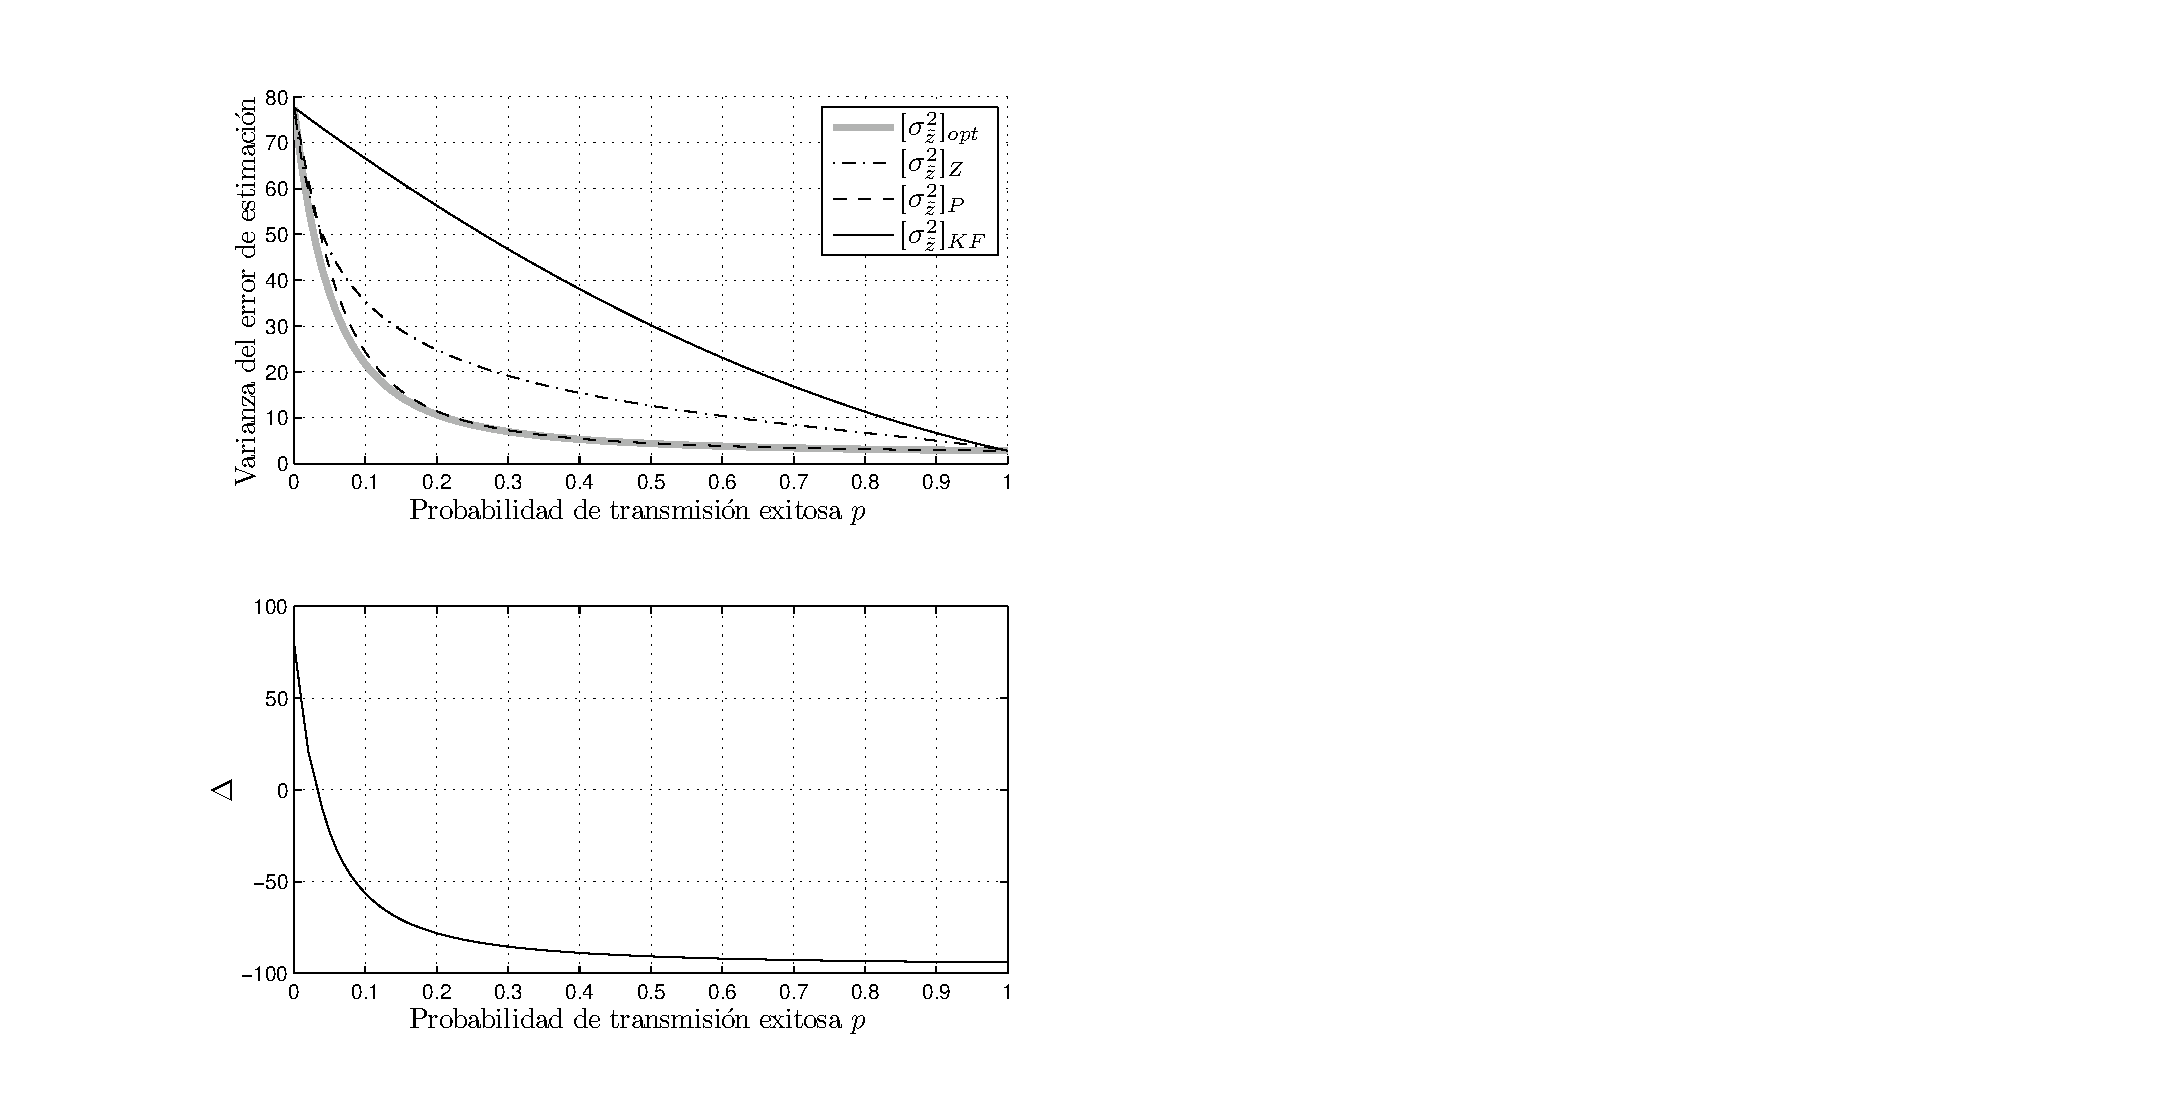
\epsfig{file=./figuras/miso.eps,width=1.6\textwidth}
\caption{Varianza del error de estimaci\'on ($\traza{P_{\tilde{z}}}$) en funci\'on de la probabilidad de transmisi\'on exitosa $p$. (Caso de salida escalar.)}
\label{fig:example-miso}
\end{figure}

Los resultados expuestos en la Figura \ref{fig:example-miso} muestran (como es de esperar), que el peor desempe\~no lo alcanza el filtro de Kalman que ha sido dise\~nado sin considerar la p\'erdida de datos. El desempe\~no de este filtro se puede mejorar tomando en cuenta esta informaci\'on en la etapa de dise\~no, y puede ser mejorado a\'un m\'as al reemplazar los datos perdidos por las muestras efectivamente recibidas en instantes anteriores. Este \'ultimo esquema de compensaci\'on se acerca al \'optimo para probabilidades $p>0.2$, y se alcanza un desempe\~no considerablemente mejor que la otra estrategia sub\'optima para probabilidades $p>0.05$.

En la Figura \ref{fig:example-miso} se muestra tambi\'en un gr\'afico para $\Delta$ (ver Corolario \ref{coro:compara}), cuyo signo determina cual estrategia sub\'optima alcanza un mejor desempe\~no. Los resultados son consistentes con los del Corolario \ref{coro:compara}.
\newpage
En segundo lugar, se consider\'o el sistema en \eqref{eq:sistema} con las matrices anteriores, excepto que $\renewcommand{\arraystretch}{0.75} A = \matriz{ 0.5 & 0 \\ 0.3 & 0.4 }$.  Dado que en este caso los autovalores de $A$ est\'an m\'as cerca del origen, uno esperar\'ia que reemplazar muestras perdidas por ceros sea una estrategia de compensaci\'on m\'as adecuada que en el caso anterior. Este hecho intuitivo se encuentra claramente respaldado por los resultados de la Figura \ref{fig:example-delta}.

\begin{figure}[htbp]
\centering
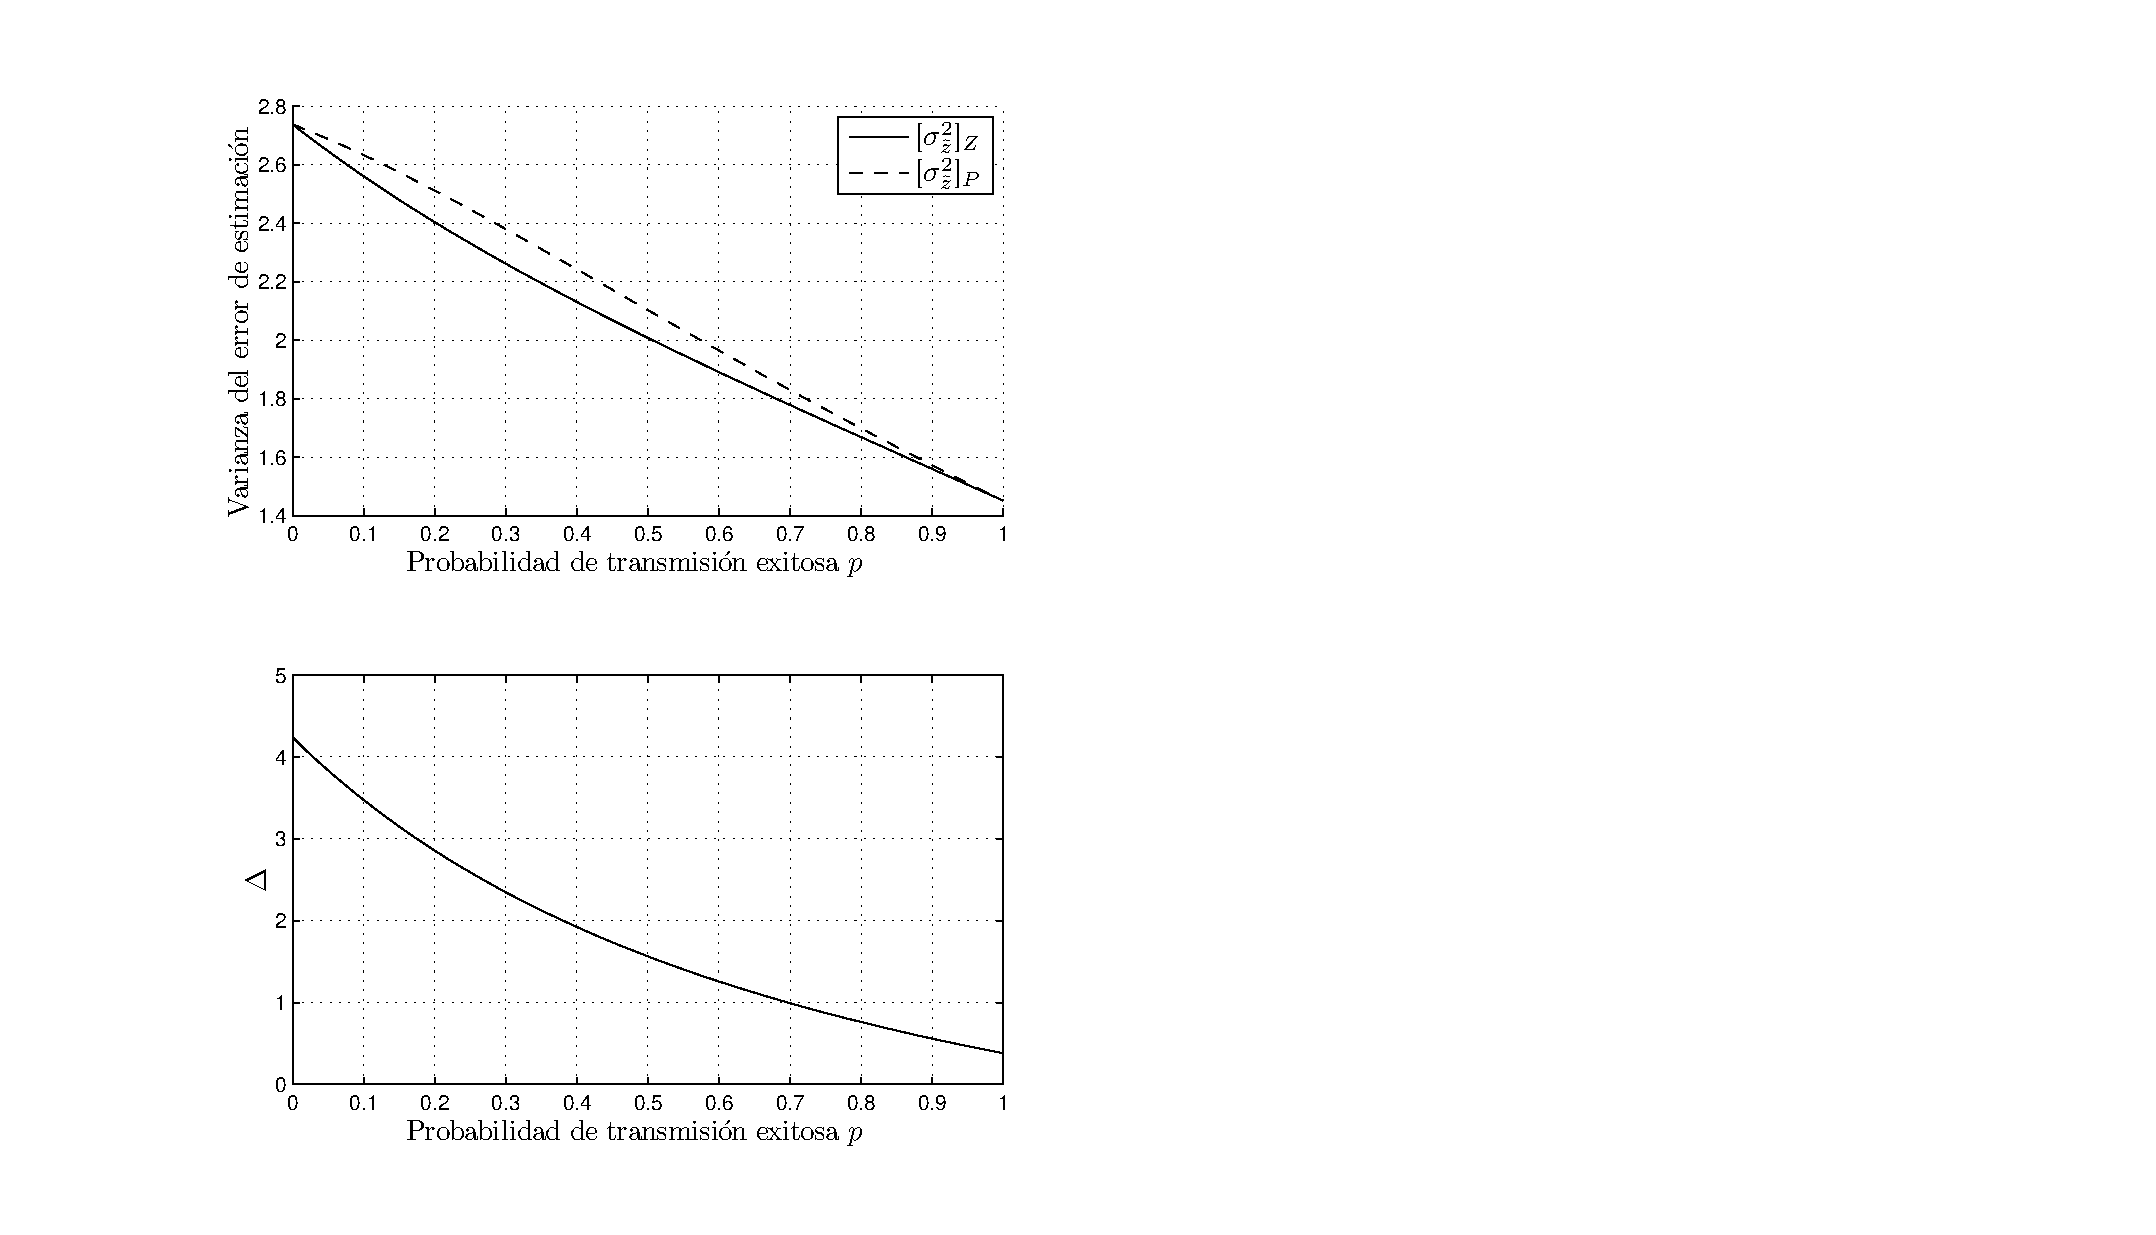
\epsfig{file=./figuras/delta.eps,width=1.4\textwidth}
\caption{Comparaci\'on entre las estrategias de compensaci\'on sub\'optimas para un sistema de salida escalar con modos naturales relativamente r\'apidos.}\label{fig:example-delta}
\end{figure}
\newpage
Finalmente, se considera un caso en que las mediciones no son escalares. Se ha supuesto que todas las matrices del sistema tienen los valores definidos en el primer ejemplo, a excepci\'on de las indicadas a continuaci\'on:
\begin{align*}
C_y = \matriz{ 1 & 1 \\ 2 & 1 }, \quad D_y = \matriz{ 0 & 0 & 1 \\ 0 & 0 & 1}.
\end{align*}
Los resultados se muestran en la Figura \ref{fig:example-mimo}, donde adem\'as se muestra el gr\'afico correspondiente a los autovalores de $\Delta$. Como es de esperar, cuando $\Delta$ es positiva definida, i.e., para $p<0.03$, el m\'etodo de reemplazar las perdidas por ceros alcanza el mejor desempe\~no dentro de las estrategias sub\'optimas consideradas. Para otros valores de $p$, $\Delta$ no es una matriz definida y, por lo tanto, no se puede anticipar ninguna conclusi\'on en forma inmediata.

\begin{figure}[htbp]
\centering
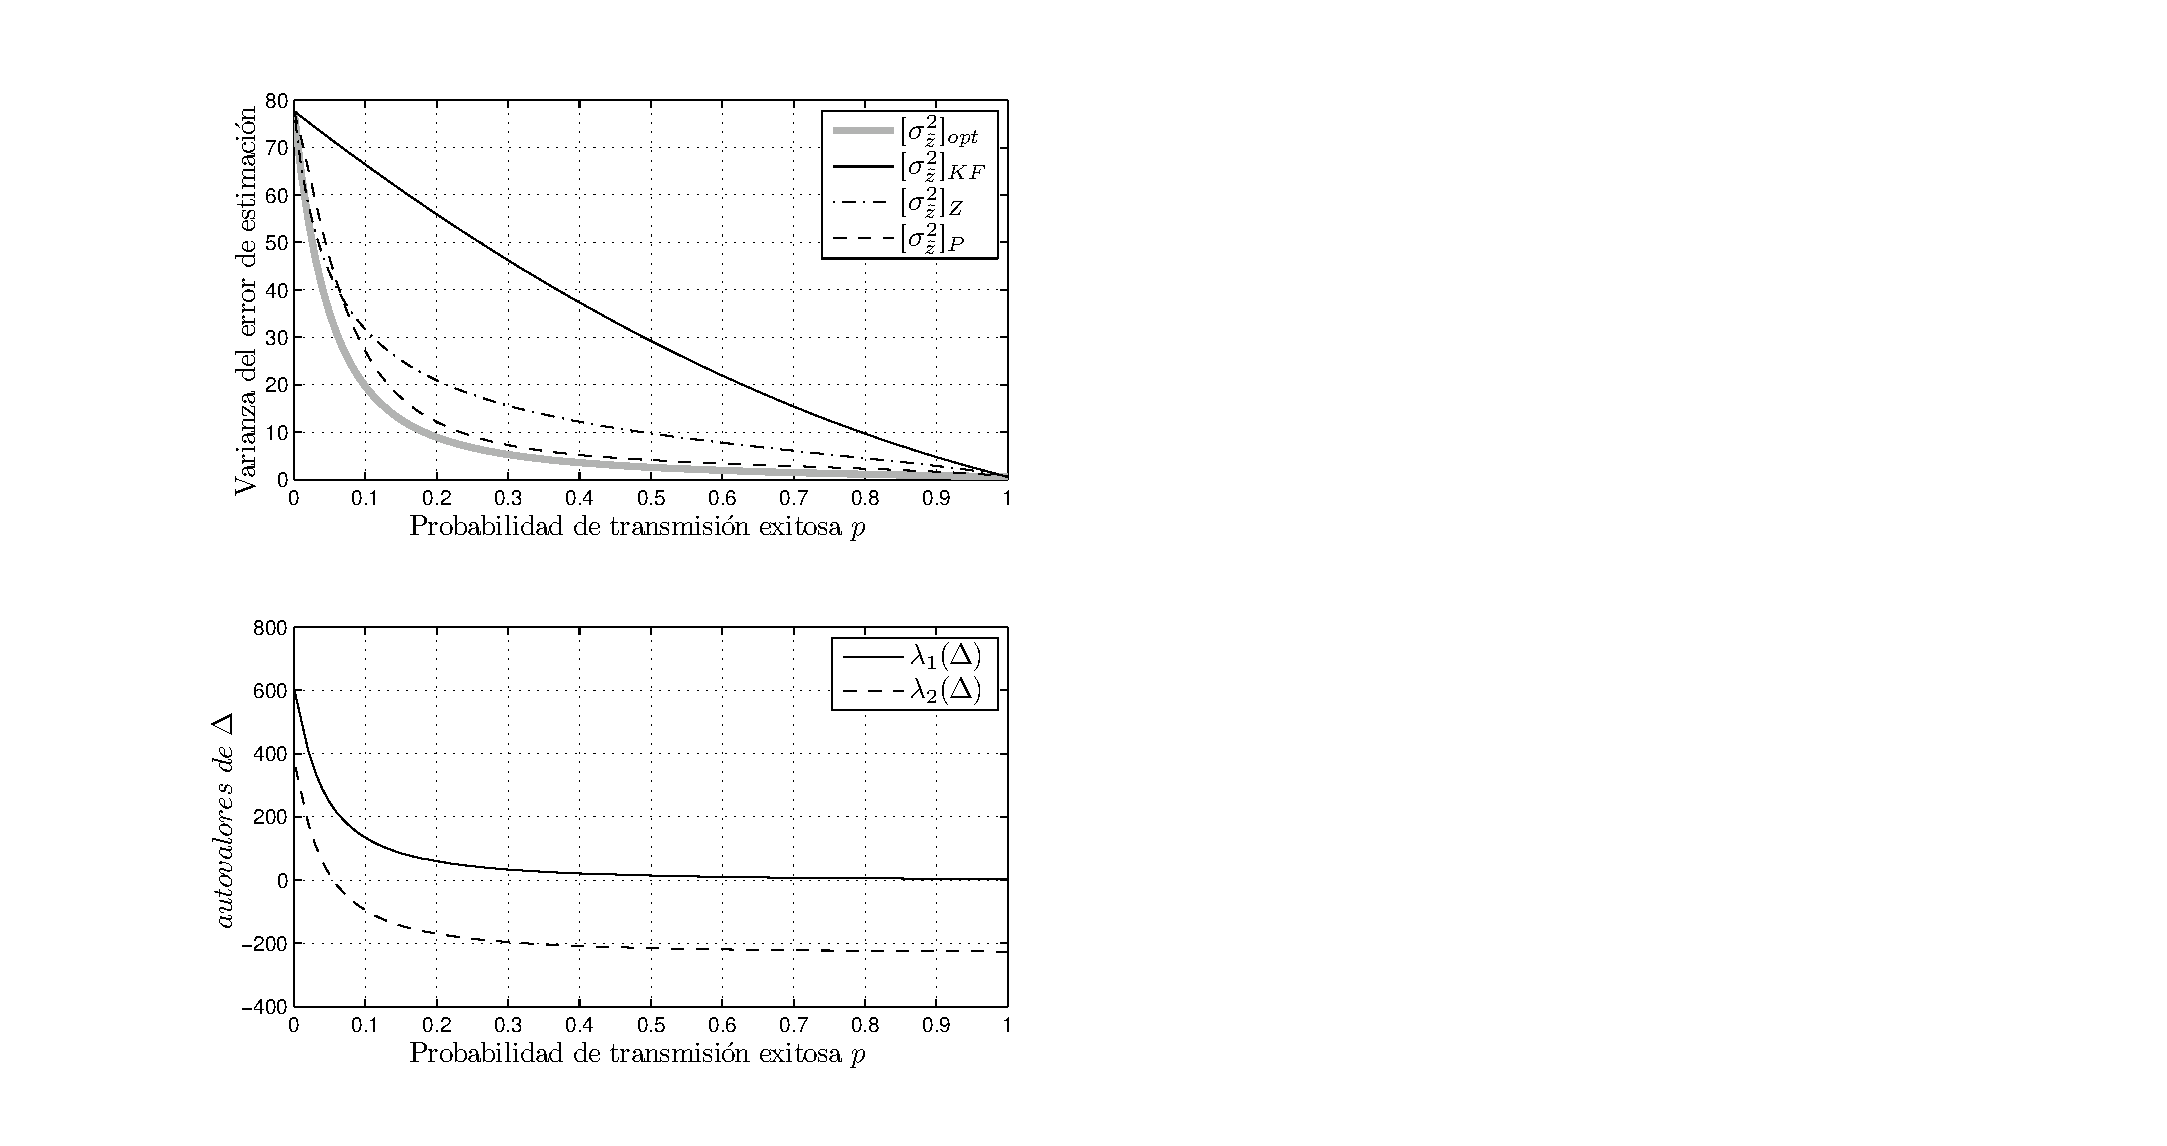
\epsfig{file=./figuras/mimo.eps,width=1.45\textwidth}
\caption{Varianza del error de estimaci\'on ($\traza{P_{\tilde{z}}}$) como funci\'on de la probabilidad de transmisi\'on exitosa $p$.( Caso de salidas m\'ultiples.)}\label{fig:example-mimo}
\end{figure}

Los resultados anteriores muestran que los esquemas de compensaci\'on de datos perdidos son esenciales para dise\~nar estimadores que alcancen un buen desempe\~no al estimar se\~nales sobre canales de borrado. A pesar de que la estrategia de reemplazar las perdidas por muestras correctamente recibidas anteriormente parece ser una opci\'on atractiva, el esquema de compensaci\'on \'optimo ac\'a propuesto ofrece un mejor desempe\~no en todo momento.

Cabe notar que el verdadero estimador \'optimo para este tipo de sistemas vendr\'ia dado por un filtro perteneciente a la clase de MJLS, el que haciendo uso de la informaci\'on acerca del estado del canal, conmuta sus par\'ametros de forma de ser sintonizado ya sea se est\'en recibiendo datos o \'estos se pierdan en el canal, donde la evoluci\'on de la varianza del error de estimaci\'on queda descrita por
\begin{equation}
P(k+1)=A_{\theta(k)}(k)P(k)A_{\theta(k)}^{\intercal}(k)+B_{\theta(k)}(k)B_{\theta(k)}^{\intercal}(k)+J(k)C_{\theta(k)}(k)P(k)A_{\theta(k)}^{\intercal}(k),
\end{equation}
donde $J(k)$ corresponde a la ganancia del Filtro de Kalman en el instante $k$, y se obtiene como
\begin{equation}
J(k)=-A_{\theta(k)}(k)P(k)C_{\theta(k)}^{\intercal}(k)\left( C_{\theta(k)}(k)P(k)C_{\theta(k)}^{\intercal}(k)+D_{y,\theta(k)}(k)D_{y,\theta(k)}^{\intercal}(k)\right)^{-1}.
\end{equation}
En la Figura \ref{fig:kf} se observa el desempeño obtenido por el estimador ac\'a propuesto, as\'i como tambi\'en se observan las cotas de \'este, notando que la cota inferior representa el mejor desempeño alcanzable, el cual viene dado por el filtro de Kalman conmutado que se mencion\'o anteriormente, notando que dada su naturaleza, \'este filtro no converge a un estimador estacionario como el propuesto.

\begin{figure}[htbp]
\centering
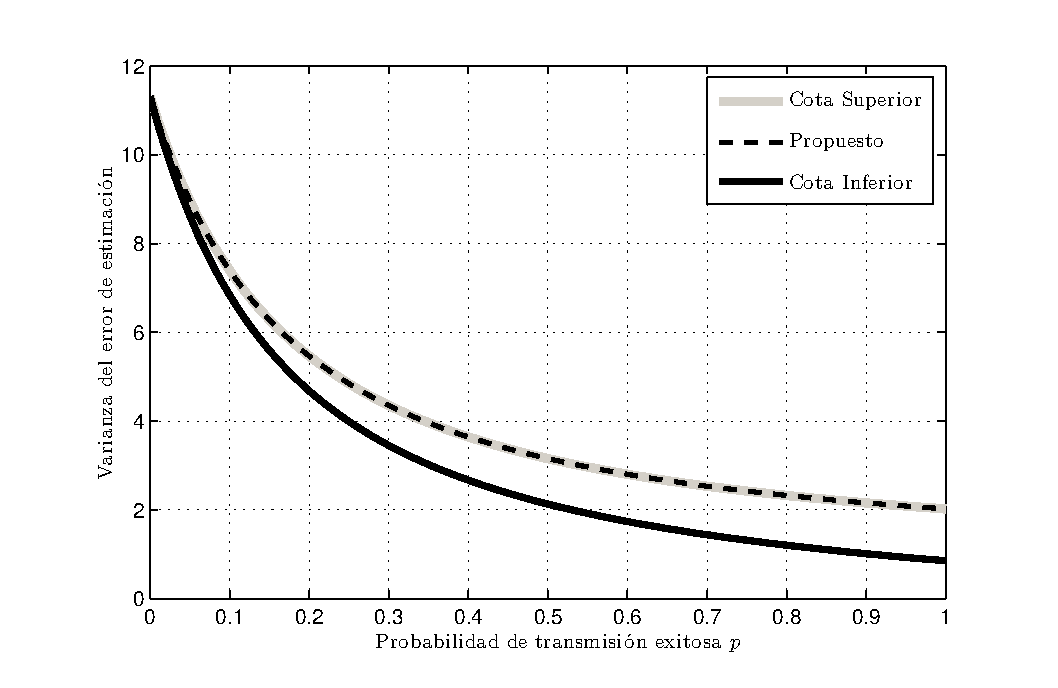
\includegraphics[scale=0.6]{./figuras/opt_kf.eps}
\caption{Comparaci\'on de estimador propuesto y cotas superior e inferior.}
\label{fig:kf}
\end{figure}

Se debe notar que, tal como se se\~nala en \cite{cofrma05,ji1990jump}, si se quisiera pre-calcular las ganancias de este Filtro de Kalman para as\'i ahorrar tiempo de computo cuando se realice la estimaci\'on en l\'inea (como se menciona en \cite{chung1976minimum}), entonces la complejidad computacional de este estimador aumenta exponencialmente acorde aumenta el horizonte de tiempo de la estimaci\'on, notando que para un intervalo $[0,T]$ ser\'ia necesario precalcular $N\frac{N^T-1}{N-1}$ ganancias.

\newpage
\section{Conclusiones}
En este cap\'itulo se ha estudiado un problema de estimaci\'on estacionaria sujeto a la p\'erdida de datos. Se ha logrado llevar dicho problema de estimaci\'on desde el sistema conmutado original, a otro sistema equivalente en segundos momentos para realizar as\'i el dise\~no del estimador \'optimo.

Se ha entregado una caracterizaci\'on expl\'icita de las variables de inter\'es, tales como la varianza del ruido auxiliar o la varianza del error de estimaci\'on, permitiendo as\'i una mayor comprensi\'on del problema y facilitando la comparaci\'on entre los distintos esquemas de compensaci\'on de p\'erdida de datos que se pueden encontrar en la literatura.

Finalmente, se han mostrado ejemplos que permiten ilustrar los resultados obtenidos a lo largo de este cap\'itulo, realizando tambi\'en una comparaci\'on entre el estimador estacionario aqu\'i propuesto y sus cotas, donde la  cota m\'inima corresponde al desempeño que logra el filtro de Kalman variante en el tiempo, siendo un estimador \'optimo que no converge a uno estacionario.
%
%%%%%%%%%%%%%%%%%%%%%%%%%%%%%%%%%%%%%%%%%%%%%%%%%%%%%%%%%%%%%%
%
\cleardoublepage
\chapter{Conclusiones}
\label{cap:conclusiones}
\section{Discusi\'on y comparaci\'on de los resultados obtenidos}
En este trabajo de tesis se ha estudiado un problema de estimaci\'on estacionaria sujeto a restricciones de comunicaci\'on. En particular, se ha estudiado un caso en que las mediciones que utiliza el filtro para realizar la estimaci\'on son enviadas a trav\'es de un canal de borrado. Esto implica que dichas mediciones podr\'ian perderse, es decir, podr\'ian no llegar al extremo receptor del canal, con cierta probabilidad. En este contexto, se puede encontrar una gran variedad de tipos de filtros, debiendo hacerse las siguientes preguntas para poder diferenciar correctamente el tipo de filtro que se tiene:
\begin{itemize}
\item ¿Es el filtro un MJLS o es un sistema LTI?.
\item ¿Se supone acceso al estado del canal?, de ser as\'i, ¿esta informaci\'on se supone de obtenci\'on inmediata o est\'a atrasada?.
\item ¿Se utiliza un esquema de compensaci\'on para los datos perdidos?
\item ¿El filtro converge a uno estacionario?.
\item ¿El filtro es \'optimo dentro de su clase?
\end{itemize}
Hacer estas diferencias es importante, ya que no es justo comparar el desempe\~no de un filtro frente a otro estimador que pertenece a una clase distinta. De esta manera es natural que, el desempe\~no del filtro desarrollado en el Capitulo \ref{cap:estimacion_mimo} no puede competir con filtros más generales, como el filtro de Kalman variante en el tiempo, donde este tipo de estimadores pertenecen a una clase m\'as amplia de filtros.

Uno de los resultados principales obtenidos en este trabajo de tesis, es la caracterizaci\'on expl\'icita de un filtro estacionario con par\'ametros dependientes del estado del canal. Dicho resultado se ha obtenido considerando un sistema auxiliar, estad\'isticamente equivalente al sistema original, en el cual resulta m\'as f\'acil realizar las tareas de an\'alisis y dise\~no. 

Otro aspecto importante a notar es la estructura del filtro obtenido en el Cap\'itulo \ref{cap:estimacion_mimo}. El problema de dise\~no se pudo separar en dos problemas consecutivos. En la primera etapa, se dise\~na un compensador de los datos perdidos. Este problema es un problema de estimaci\'on \'optima sujeto a una restricci\'on de SNR. El segundo paso, corresponde a un problema de filtraje est\'andar en el que surge una fuente de ruido auxiliar cuya varianza depende del compensador de p\'erdidas utilizado.

Otro resultado importante corresponde a la obtenci\'on de expresiones cerradas que caracterizan la varianza \'optima del ruido auxiliar en el caso de que las mediciones correspondan a una se\~nal escalar. Esto permite analizar de forma inmediata los efectos de los par\'ametros del sistema sobre los resultados obtenidos. De la misma forma, fue posible obtener una expresi\'on muy simple para la m\'inima varianza del error de estimaci\'on en el caso en que la se\~nal que interesa estimar es escalar y corresponde a la misma se\~nal que se env\'ia a trav\'es del canal de borrado. Este caso que parece muy particular, puede resultar de cierto inter\'es para aplicaciones que involucren, por ejemplo, procesamiento de audio, en que se env\'ia cierto sonido y a partir de las mismas mediciones de \'este, se quiere reconstruir el sonido original dado que se perdieron algunas muestras.

Finalmente, fue posible realizar una comparaci\'on entre las estrategias de compensaci\'on de p\'erdida de datos que se han propuesto con mayor frecuencia en la literatura. Se entregan condiciones que garantizan que una de estas estrategias es superior a la otra. En particular, cuando la medici\'on enviada a trav\'es del canal corresponde a una se\~nal escalar, se pueden obtener condiciones necesarias y suficientes, pero cuando esta se\~nal contiene m\'ultiples mediciones, s\'olo se pueden obtener condiciones necesarias.

Con el desarrollo realizado, y en particular con la observaci\'on que involucra la separaci\'on del problema original en dos partes, se mostr\'o que el desempe\~no que logra cierto estimador tiene directa relaci\'on con la estrategia de compensaci\'on para la p\'erdida de datos que se est\'e utilizando. Es relevante notar que un mejor esquema de compensaci\'on, es decir, aquel compensador que involucre una menor varianza para el ruido auxiliar, permitir\'a obtener mejores estimaciones.

\section{Trabajo futuro}
Dados los resultados obtenidos en este trabajo de tesis, consideramos que los siguientes son temas para trabajo futuro.
\begin{itemize}
\item Extender el desarrollo realizado en este documento, al caso en que se env\'ian m\'ultiples mediciones a trav\'es de m\'ultiples canales.
\item Estudiar el caso de estimaci\'on estacionaria de estado sujeto a p\'erdida de datos en el (los) canal(es), dado que la planta a considerar es de naturaleza inestable. En este caso se espera que un desarrollo no tan complejo entregue condiciones bajo las cuales se pueda proveer de una estimaci\'on con estad\'isticas de segundo orden finitas, para ciertas probabilidades de transmisi\'on $p$.
\item Analizar el problema estudiado en este trabajo de tesis, para el caso en que coexisten diversas restricciones de comunicaci\'on en el (los) canal(es) presente(s). Por ejemplo, puede ser de inter\'es el caso en que la se\~nal que se env\'ia a trav\'es del canal de borrado ha sido previamente cuantizada.
\end{itemize} 
%
%%%%%%%%%%%%%%%%%%%%%%%%%%%%%%%%%%%%%%%%%%%%%%%%%%%%%%%%%%%%%%
%
%%------------------AP\'eNDICES--------------------------------
%
%%%%%%%%%%%%%%%%%%%%%%%%%%%%%%%%%%%%%%%%%%%%%%%%%%%%%%%%%%%%%

\cleardoublepage
\appendix
\chapter{Ap\'endice}
\label{cap:apendice}
\input apendice1.tex
\chapter{Notaci\'on}
\label{cap:notacion}
\input apendice2.tex


%------------------BIBLIOGRAF\'iA-----------------------------

\bibliographystyle{plain}
\bibliography{bib}

\end{document}